% ============================================================
% RAPPORT DE PROJET HUBFPK
% Module : Citoyenneté et Initiation
% Professeur : M. CHAKRAOUI Mohamed
% ============================================================
\documentclass[12pt, a4paper]{report}

% ---------- Encodage et Langue ----------
\usepackage[utf8]{inputenc}
\usepackage[T1]{fontenc}
\usepackage[french]{babel}

% ---------- Police personnalisée ----------
\usepackage{charter}            % Police Charter (serif élégante)
\usepackage[scaled=0.92]{helvet} % Helvetica pour le sans-serif
\usepackage{inconsolata}        % Police pour le code

% ---------- Mise en page ----------
\usepackage[top=2.5cm, bottom=2.5cm, left=2.5cm, right=2.5cm]{geometry}
\usepackage{setspace}
\onehalfspacing

% ---------- Graphiques et Images ----------
\usepackage{graphicx}
\usepackage{float}
\usepackage{subcaption}

% ---------- Couleurs et Liens ----------
\usepackage[dvipsnames]{xcolor}

% Couleur personnalisée HubFPK
\definecolor{HubGreen}{HTML}{1a5c3a}
\definecolor{HubAmber}{HTML}{FBBF24}

\usepackage{hyperref}
\hypersetup{
    colorlinks=true,
    linkcolor=HubGreen,
    citecolor=HubGreen,
    urlcolor=HubGreen,
    pdfauthor={HABYBY Zahira, EL MAHI Nadia, EL HOSSI Fatima Zahra, ANAM Ayoub},
    pdftitle={Rapport de Projet HubFPK},
}

% ---------- Tableaux et Listes ----------
\usepackage{booktabs}
\usepackage{array}
\usepackage{enumitem}
\usepackage{longtable}
\usepackage{tabularx}

% ---------- Code Source ----------
\usepackage{listings}
\lstset{
    basicstyle=\small\ttfamily,
    keywordstyle=\bfseries\color{HubGreen},
    commentstyle=\itshape\color{gray},
    stringstyle=\color{OliveGreen},
    numbers=left,
    numberstyle=\tiny\color{gray},
    numbersep=8pt,
    frame=single,
    rulecolor=\color{gray!30},
    backgroundcolor=\color{gray!5},
    breaklines=true,
    breakatwhitespace=true,
    tabsize=4,
    showstringspaces=false,
    captionpos=b,
}

% ---------- En-têtes et Pieds de page ----------
\usepackage{fancyhdr}
\pagestyle{fancy}
\fancyhf{}
\fancyhead[L]{\leftmark}
\fancyhead[R]{\thepage}
\renewcommand{\headrulewidth}{0.4pt}
\fancyfoot[C]{\footnotesize HubFPK -- Citoyenneté et Initiation}
\renewcommand{\footrulewidth}{0.2pt}

% ---------- Titres personnalisés ----------
\usepackage{titlesec}
\titleformat{\chapter}[display]
  {\normalfont\huge\bfseries\sffamily\color{HubGreen}}
  {\chaptertitlename\ \thechapter}{20pt}{\Huge}
\titleformat{\section}
  {\normalfont\Large\bfseries\sffamily\color{HubGreen!90!black}}
  {\thesection}{1em}{}
\titleformat{\subsection}
  {\normalfont\large\bfseries\sffamily\color{HubGreen!80!black}}
  {\thesubsection}{1em}{}

% ---------- Divers ----------
\usepackage{parskip}
\usepackage{caption}
\captionsetup{font=small, labelfont=bf, labelsep=period}

% ============================================================
%                      DÉBUT DU DOCUMENT
% ============================================================
\begin{document}

% ==================== PAGE DE GARDE ====================
\begin{titlepage}
    % --- LOGOS ---
    \noindent
    
\includegraphics[height=2.2cm]{logo_usms}%
    \hfill
    
\includegraphics[height=2.2cm]{logo_FPK}\par%
    
    \vspace{1cm}
    
    \centering
    
    {\Large\sffamily\bfseries Université Sultan Moulay Slimane\par}
    \vspace{0.3cm}
    {\large\sffamily Master d'Excellence SiiA\par}
    
    \vspace{2cm}
    
    \rule{\textwidth}{1.5pt}\\[0.5cm]
    {\fontsize{36}{42}\selectfont\sffamily\bfseries\color{HubGreen} Hub\textcolor{HubAmber}{FPK}}\\[0.3cm]
    {\Large\sffamily Plateforme Communautaire Full-Stack pour la Faculté Polydisciplinaire de Khouribga}\\[0.5cm]
    \rule{\textwidth}{1.5pt}
    
    \vspace{1.5cm}
    
    {\large\sffamily\bfseries Module :} {\large\sffamily Citoyenneté et Initiation}\\[0.3cm]
    {\large\sffamily\bfseries Encadré par :} {\large\sffamily M. CHAKRAOUI Mohamed}
    
    \vspace{2cm}
    
    {\large\sffamily\bfseries Réalisé par :}\\[0.4cm]
    \begin{tabular}{l}
        \large\sffamily HABYBY Zahira \\
        \large\sffamily EL MAHI Nadia \\
        \large\sffamily EL HOSSI Fatima Zahra \\
        \large\sffamily ANAM Ayoub \\
    \end{tabular}
    
    \vfill
    
    {\large\sffamily Année universitaire 2025 / 2026}
\end{titlepage}

% ==================== TABLE DES MATIÈRES ====================
\tableofcontents
\newpage

% ============================================================
% CHAPITRE 1 : INTRODUCTION GÉNÉRALE
% ============================================================
\chapter{Introduction Générale}

\section{Contexte du Projet}

Dans le paysage universitaire marocain, et plus particulièrement au sein de la Faculté Polydisciplinaire de Khouribga (FPK), les étudiants font face à un manque criant d'espaces numériques dédiés à l'entraide, au partage de connaissances et à la communication entre pairs. Les canaux existants -- groupes WhatsApp éphémères, pages Facebook non structurées -- ne permettent pas de capitaliser sur les questions posées, les réponses apportées ou les ressources partagées. L'information se perd, les mêmes questions sont posées chaque année, et aucune mémoire collective ne se constitue.

C'est dans ce contexte que le projet \textbf{HubFPK} a été conçu : une plateforme communautaire \textit{full-stack} inspirée des forums modernes, pensée pour centraliser les échanges académiques des étudiants de la FPK dans un environnement structuré, ergonomique et pérenne.

\section{Problématique}

Comment offrir aux étudiants de la FPK un espace numérique structuré, accessible et engageant qui permette de :
\begin{itemize}[leftmargin=2cm]
    \item Centraliser les discussions par département académique ?
    \item Valoriser les contributions de qualité grâce à un système de réputation ?
    \item Offrir des notifications en temps réel pour maintenir l'engagement ?
    \item Garantir une modération naturelle via le système de votes communautaires ?
\end{itemize}

\section{Objectifs du Projet}

Le projet HubFPK poursuit plusieurs objectifs fondamentaux :

\begin{itemize}[leftmargin=2cm]
    \item[\textbf{1.}] \textbf{Créer un forum communautaire moderne} organisé par départements académiques (Informatique, Mathématiques, Économie, Sciences, Langues, Vie étudiante, Annonces).
    \item[\textbf{2.}] \textbf{Implémenter un système de vote et de karma} similaire à celui de Reddit, permettant aux étudiants de valoriser les contributions pertinentes.
    \item[\textbf{3.}] \textbf{Offrir un éditeur Markdown} pour que les étudiants puissent rédiger des publications riches et bien formatées (code, formules, liens).
    \item[\textbf{4.}] \textbf{Développer un système de notifications en temps réel} via les WebSockets de Supabase Realtime.
    \item[\textbf{5.}] \textbf{Déployer l'application en production} sur Vercel pour la rendre accessible à tous les étudiants.
\end{itemize}

\section{Sources d'Inspiration}

La conception de HubFPK s'est largement inspirée de plateformes communautaires à succès qui ont révolutionné la manière dont les communautés en ligne interagissent :

\subsection{Reddit}

\textbf{Reddit} (fondé en 2005) est la plus grande plateforme communautaire au monde, avec plus de 1,7 milliard d'utilisateurs actifs mensuels. Son modèle repose sur des \textit{subreddits} (sous-communautés thématiques), un système de votes \textit{upvote/downvote}, et un système de \textit{karma} qui récompense les contributions de qualité. HubFPK reprend ces concepts fondamentaux :

\begin{itemize}
    \item \textbf{Catégories} $\rightarrow$ équivalent des subreddits de Reddit
    \item \textbf{Système de votes ±1} $\rightarrow$ inspiré du upvote/downvote
    \item \textbf{Karma utilisateur} $\rightarrow$ directement inspiré du karma Reddit
    \item \textbf{Fils de discussion avec réponses imbriquées} $\rightarrow$ modèle Reddit de commentaires
\end{itemize}

\subsection{Stack Overflow}

\textbf{Stack Overflow} est la référence mondiale pour les questions-réponses techniques. HubFPK s'en inspire pour :

\begin{itemize}
    \item \textbf{Le système de tags} (Question, Discussion, Ressource, Annonce) pour catégoriser le contenu
    \item \textbf{Le support du Markdown} pour le formatage des publications
    \item \textbf{Le compteur de vues} pour mesurer la popularité des sujets
\end{itemize}

\subsection{Discourse}

\textbf{Discourse} est une plateforme de forum open-source moderne qui a inspiré HubFPK pour :

\begin{itemize}
    \item \textbf{Le design épuré et moderne} avec des catégories visuelles colorées
    \item \textbf{Les notifications en temps réel} sans rechargement de page
    \item \textbf{L'accent sur la communauté} avec des profils utilisateurs riches
\end{itemize}

\section{Structure du Rapport}

Ce rapport est organisé de la manière suivante :
\begin{itemize}
    \item Le \textbf{Chapitre 2} présente l'architecture technique globale du projet.
    \item Le \textbf{Chapitre 3} détaille la conception de la base de données.
    \item Le \textbf{Chapitre 4} décrit le backend API REST et ses endpoints.
    \item Le \textbf{Chapitre 5} présente le frontend React et l'interface utilisateur.
    \item Le \textbf{Chapitre 6} aborde le déploiement en production sur Vercel.
    \item Le \textbf{Chapitre 7} conclut le rapport avec un bilan et des perspectives d'amélioration.
\end{itemize}


% ============================================================
% CHAPITRE 2 : ARCHITECTURE TECHNIQUE
% ============================================================
\chapter{Architecture Technique}

\section{Vue d'Ensemble}

HubFPK repose sur une architecture \textbf{Full-Stack découplée} composée de trois couches distinctes, communiquant entre elles via des API REST et le protocole WebSocket :

\begin{enumerate}
    \item \textbf{La couche de présentation} : Application React (Vite) côté client.
    \item \textbf{La couche métier} : API REST Node.js/Express servant d'intermédiaire.
    \item \textbf{La couche de données} : Base de données PostgreSQL hébergée sur Supabase.
\end{enumerate}

\section{Diagramme d'Architecture}

Le flux de données suit le schéma suivant :

\begin{verbatim}
[Client React/Vite] ──────► [Backend Express.js] ──────► [Supabase (PostgreSQL)]
       │                                                          ▲
       └──────────────── (Supabase JS Client) ────────────────────┘
                    (Auth, Realtime, opérations directes)
\end{verbatim}

Cette architecture présente une particularité intéressante : il existe une \textbf{double voie d'accès à la base de données}. Le frontend communique avec le backend Express pour la majorité des opérations de lecture, mais utilise également le client Supabase JS directement pour l'authentification, les votes et les notifications en temps réel.

\section{Stack Technologique}

\begin{table}[H]
\centering
\renewcommand{\arraystretch}{1.4}
\begin{tabularx}{\textwidth}{>{\bfseries}l X}
\toprule
\textbf{Composant} & \textbf{Technologies Utilisées} \\
\midrule
Base de données & PostgreSQL (via Supabase) avec Row Level Security (RLS) \\
Backend \& API & Node.js, Express 5.2, @supabase/supabase-js 2.99, dotenv, cors \\
Frontend & React 19, Vite 8, React Router DOM 7.13, TailwindCSS 4.2 \\
Éditeur de contenu & react-markdown 10.1 (rendu Markdown) \\
Temps réel & Supabase Realtime (WebSocket / postgres\_changes) \\
Icônes & Lucide React 0.577 (bibliothèque d'icônes SVG) \\
Utilitaires & axios 1.13, date-fns 4.1, clsx, tailwind-merge \\
Hébergement & Vercel (Frontend + Backend en Serverless Functions) \\
\bottomrule
\end{tabularx}
\caption{Résumé complet de la stack technologique du projet HubFPK.}
\end{table}

\section{Flux de Données}

Le flux de données typique d'un utilisateur suit le cheminement suivant :

\begin{enumerate}
    \item L'étudiant s'inscrit et se connecte via \textbf{Supabase Auth} (email + mot de passe). Un profil est automatiquement créé grâce à un trigger PostgreSQL.
    \item Les opérations de \textbf{lecture} (catégories, threads, profils, stats) passent par l'\textbf{API Express} via des appels \texttt{axios}.
    \item Les opérations d'\textbf{écriture} (votes, posts) utilisent tantôt l'API Express, tantôt le \textbf{client Supabase JS} côté frontend.
    \item Les \textbf{notifications en temps réel} sont reçues via les \texttt{Realtime Channels} de Supabase (protocole WebSocket), sans aucun polling.
    \item L'API Express communique avec Supabase via le \textbf{Service Role Key} (clé avec droits administratifs), contournant le RLS côté serveur.
\end{enumerate}


% ============================================================
% CHAPITRE 3 : BASE DE DONNÉES
% ============================================================
\chapter{Conception de la Base de Données}

\section{Choix de Supabase}

Le projet utilise \textbf{Supabase} comme Backend-as-a-Service (BaaS). Supabase est une alternative open-source à Firebase, offrant :

\begin{itemize}
    \item Une base de données \textbf{PostgreSQL} complète (relationnelle, avec support des UUID, JSON, triggers).
    \item Un système d'\textbf{authentification} intégré (email/password, OAuth, Magic Links).
    \item Des \textbf{Realtime Channels} pour écouter les changements en base de données via WebSocket.
    \item Un système de \textbf{Row Level Security (RLS)} pour sécuriser l'accès aux données au niveau SQL.
    \item Des \textbf{Stored Procedures} appelables via RPC depuis le client.
\end{itemize}

\section{Schéma Relationnel}

La base de données est structurée autour de six tables principales, interconnectées par des clés étrangères :

\begin{verbatim}
auth.users (Supabase Built-in)
     │
     ▼
profiles (id PK → auth.users)
     │
     ├──► threads (user_id FK)
     │         │
     │         ├──► posts (thread_id FK)
     │         │       └──► posts (parent_post_id FK — nesting 1 niveau)
     │         │
     │         └──► votes (target_id polymorphe)
     │
     └──► notifications (user_id FK)

categories ──► threads (category_id FK)
\end{verbatim}

\section{Description Détaillée des Tables}

\subsection{Table \texttt{profiles}}

Cette table étend la table interne \texttt{auth.users} de Supabase. Chaque nouvel utilisateur inscrit voit son profil automatiquement créé grâce au trigger \texttt{handle\_new\_user()}.

\begin{table}[H]
\centering
\renewcommand{\arraystretch}{1.3}
\begin{tabularx}{\textwidth}{l l X}
\toprule
\textbf{Colonne} & \textbf{Type} & \textbf{Description} \\
\midrule
\texttt{id} & UUID & Clé primaire, FK vers \texttt{auth.users} \\
\texttt{username} & TEXT & Nom d'utilisateur unique \\
\texttt{avatar\_url} & TEXT & URL de l'avatar \\
\texttt{bio} & TEXT & Biographie de l'étudiant \\
\texttt{karma} & INTEGER & Score de réputation (défaut : 0) \\
\texttt{created\_at} & TIMESTAMPTZ & Date d'inscription \\
\bottomrule
\end{tabularx}
\caption{Structure de la table \texttt{profiles}.}
\end{table}

\subsection{Table \texttt{categories}}

Contient les 7 départements académiques de la FPK. Les catégories sont pré-remplies (\textit{seed data}) lors de l'initialisation de la base.

\begin{table}[H]
\centering
\renewcommand{\arraystretch}{1.3}
\begin{tabularx}{\textwidth}{l l X}
\toprule
\textbf{Colonne} & \textbf{Type} & \textbf{Description} \\
\midrule
\texttt{id} & UUID & Clé primaire auto-générée \\
\texttt{name} & TEXT & Nom du département \\
\texttt{slug} & TEXT & Identifiant URL-friendly (unique) \\
\texttt{description} & TEXT & Description du département \\
\texttt{icon} & TEXT & Nom de l'icône Lucide associée \\
\bottomrule
\end{tabularx}
\caption{Structure de la table \texttt{categories}.}
\end{table}

Les 7 catégories sont : \textbf{Informatique}, \textbf{Mathématiques}, \textbf{Économie}, \textbf{Langues}, \textbf{Sciences}, \textbf{Vie étudiante} et \textbf{Annonces}.

\subsection{Table \texttt{threads}}

Représente les fils de discussion créés par les étudiants.

\begin{table}[H]
\centering
\renewcommand{\arraystretch}{1.3}
\begin{tabularx}{\textwidth}{l l X}
\toprule
\textbf{Colonne} & \textbf{Type} & \textbf{Description} \\
\midrule
\texttt{id} & UUID & Clé primaire \\
\texttt{title} & TEXT & Titre du sujet (obligatoire) \\
\texttt{body} & TEXT & Corps du message (Markdown supporté) \\
\texttt{category\_id} & UUID & FK vers \texttt{categories} \\
\texttt{user\_id} & UUID & FK vers \texttt{profiles} (auteur) \\
\texttt{tag} & TEXT & Tag de type : Question, Discussion, Ressource, Annonce \\
\texttt{view\_count} & INTEGER & Nombre de consultations (défaut : 0) \\
\texttt{is\_pinned} & BOOLEAN & Épinglé en haut de liste (défaut : false) \\
\texttt{created\_at} & TIMESTAMPTZ & Date de création \\
\bottomrule
\end{tabularx}
\caption{Structure de la table \texttt{threads}.}
\end{table}

\subsection{Table \texttt{posts}}

Stocke les réponses aux threads. Supporte un niveau d'imbrication grâce à la colonne auto-référentielle \texttt{parent\_post\_id}.

\begin{table}[H]
\centering
\renewcommand{\arraystretch}{1.3}
\begin{tabularx}{\textwidth}{l l X}
\toprule
\textbf{Colonne} & \textbf{Type} & \textbf{Description} \\
\midrule
\texttt{id} & UUID & Clé primaire \\
\texttt{content} & TEXT & Contenu de la réponse (obligatoire) \\
\texttt{thread\_id} & UUID & FK vers \texttt{threads} \\
\texttt{user\_id} & UUID & FK vers \texttt{profiles} (auteur) \\
\texttt{parent\_post\_id} & UUID & FK vers \texttt{posts} (auto-ref, 1 niveau max) \\
\texttt{created\_at} & TIMESTAMPTZ & Date de publication \\
\bottomrule
\end{tabularx}
\caption{Structure de la table \texttt{posts}.}
\end{table}

\subsection{Table \texttt{votes}}

Implémente le système de vote inspiré de Reddit. Chaque utilisateur ne peut voter qu'une seule fois par élément (contrainte \texttt{UNIQUE}).

\begin{table}[H]
\centering
\renewcommand{\arraystretch}{1.3}
\begin{tabularx}{\textwidth}{l l X}
\toprule
\textbf{Colonne} & \textbf{Type} & \textbf{Description} \\
\midrule
\texttt{id} & UUID & Clé primaire \\
\texttt{user\_id} & UUID & FK vers \texttt{profiles} \\
\texttt{target\_id} & UUID & ID polymorphe (thread ou post) \\
\texttt{target\_type} & TEXT & CHECK : \texttt{'post'} ou \texttt{'thread'} \\
\texttt{value} & INTEGER & CHECK : \texttt{1} (upvote) ou \texttt{-1} (downvote) \\
\texttt{UNIQUE} & --- & Contrainte \texttt{(user\_id, target\_id)} \\
\bottomrule
\end{tabularx}
\caption{Structure de la table \texttt{votes}.}
\end{table}

\subsection{Table \texttt{notifications}}

Stocke les notifications générées automatiquement par les triggers SQL ou par le backend.

\begin{table}[H]
\centering
\renewcommand{\arraystretch}{1.3}
\begin{tabularx}{\textwidth}{l l X}
\toprule
\textbf{Colonne} & \textbf{Type} & \textbf{Description} \\
\midrule
\texttt{id} & UUID & Clé primaire \\
\texttt{user\_id} & UUID & FK vers \texttt{profiles} (destinataire) \\
\texttt{type} & TEXT & Type : \texttt{'reply'} ou \texttt{'vote'} \\
\texttt{reference\_id} & UUID & ID du thread ou post concerné \\
\texttt{is\_read} & BOOLEAN & Marqueur de lecture (défaut : false) \\
\texttt{created\_at} & TIMESTAMPTZ & Date de création \\
\bottomrule
\end{tabularx}
\caption{Structure de la table \texttt{notifications}.}
\end{table}

\section{Fonctions et Triggers SQL}

\begin{table}[H]
\centering
\renewcommand{\arraystretch}{1.3}
\begin{tabularx}{\textwidth}{l l X}
\toprule
\textbf{Fonction / Trigger} & \textbf{Déclencheur} & \textbf{Action} \\
\midrule
\texttt{handle\_new\_user()} & AFTER INSERT ON \texttt{auth.users} & Crée automatiquement un profil avec le nom d'utilisateur extrait de l'email \\
\texttt{increment\_karma()} & Appel RPC manuel & Incrémente ou décrémente le karma d'un utilisateur \\
\texttt{handle\_new\_notification()} & AFTER INSERT ON \texttt{posts} et \texttt{votes} & Génère des notifications automatiques pour les auteurs de contenu \\
\bottomrule
\end{tabularx}
\caption{Fonctions et triggers SQL du projet HubFPK.}
\end{table}

\section{Sécurité : Row Level Security (RLS)}

Toutes les tables sont protégées par le système RLS de PostgreSQL. Les politiques de sécurité définies sont :

\begin{table}[H]
\centering
\renewcommand{\arraystretch}{1.3}
\begin{tabularx}{\textwidth}{l c c}
\toprule
\textbf{Table} & \textbf{Lecture publique} & \textbf{Écriture authentifiée} \\
\midrule
\texttt{profiles} & \checkmark & Propriétaire uniquement \\
\texttt{categories} & \checkmark & Non défini \\
\texttt{threads} & \checkmark & Auteur uniquement \\
\texttt{posts} & \checkmark & Auteur uniquement \\
\texttt{votes} & \checkmark & Propriétaire uniquement \\
\texttt{notifications} & Privé & Propriétaire uniquement \\
\bottomrule
\end{tabularx}
\caption{Politiques de Row Level Security (RLS) par table.}
\end{table}


% ============================================================
% CHAPITRE 4 : BACKEND — API REST
% ============================================================
\chapter{Le Backend : API REST Express.js}

\section{Présentation Générale}

Le backend de HubFPK est une API REST développée en \textbf{Node.js} avec le framework \textbf{Express.js} (version 5.2). Il sert de couche intermédiaire entre le frontend React et la base de données Supabase. L'API est structurée en \textbf{7 modules de routes}, chacun responsable d'un domaine fonctionnel.

Le serveur écoute sur le port configurable via la variable d'environnement \texttt{PORT} (défaut : 4000) et applique un middleware CORS restreint au domaine du frontend.

\section{Structure des Fichiers}

\begin{table}[H]
\centering
\renewcommand{\arraystretch}{1.3}
\begin{tabularx}{\textwidth}{l X}
\toprule
\textbf{Fichier} & \textbf{Rôle} \\
\midrule
\texttt{index.js} & Point d'entrée du serveur, configuration des middlewares et montage des routes \\
\texttt{routes/categories.js} & CRUD des catégories (départements) \\
\texttt{routes/threads.js} & CRUD des fils de discussion avec votes et recherche \\
\texttt{routes/posts.js} & Création de réponses avec notifications \\
\texttt{routes/votes.js} & Système de vote toggle (créer/supprimer/inverser) \\
\texttt{routes/profiles.js} & Profils utilisateurs et leaderboard karma \\
\texttt{routes/notifications.js} & Récupération et marquage des notifications \\
\texttt{routes/stats.js} & Statistiques globales de la plateforme \\
\bottomrule
\end{tabularx}
\caption{Structure des fichiers du backend API.}
\end{table}

\section{Détail des Endpoints}

\subsection{Catégories (\texttt{/api/categories})}

\begin{itemize}
    \item \textbf{GET /api/categories} : Récupère toutes les catégories triées par nom et enrichit chaque catégorie avec le \textbf{nombre de threads} associés (calculé en parallèle via \texttt{Promise.all()}).
    \item \textbf{GET /api/categories/:slug} : Récupère une catégorie par son slug unique avec le comptage de threads.
\end{itemize}

\subsection{Threads (\texttt{/api/threads})}

\begin{itemize}
    \item \textbf{GET /api/threads} : Liste tous les fils de discussion avec filtrage optionnel par \texttt{category\_id} et recherche \texttt{ilike} sur le titre. Les threads épinglés apparaissent en premier, suivis des plus récents. Les votes sont récupérés en une seule requête batch.
    \item \textbf{GET /api/threads/:id} : Récupère un thread complet avec : profil de l'auteur, catégorie, tous les posts (avec profils des répondeurs), et votes. Le \textbf{compteur de vues} (\texttt{view\_count}) est incrémenté à chaque visite.
    \item \textbf{POST /api/threads} : Crée un nouveau fil de discussion.
\end{itemize}

\subsection{Posts (\texttt{/api/posts})}

\begin{itemize}
    \item \textbf{POST /api/posts} : Crée une nouvelle réponse à un thread. Si l'auteur de la réponse est différent de l'auteur du thread, une \textbf{notification automatique} de type \texttt{'reply'} est envoyée.
\end{itemize}

\subsection{Votes (\texttt{/api/votes})}

\begin{itemize}
    \item \textbf{POST /api/votes} : Implémente une logique de \textbf{vote toggle} :
    \begin{enumerate}
        \item Si l'utilisateur a déjà voté avec la \textbf{même valeur} $\rightarrow$ le vote est \textbf{supprimé} (toggle off).
        \item Si l'utilisateur a voté avec une \textbf{valeur différente} $\rightarrow$ le vote est \textbf{mis à jour}.
        \item Si aucun vote n'existe $\rightarrow$ le vote est \textbf{créé}.
    \end{enumerate}
    En cas d'upvote (\texttt{value = 1}), une notification est envoyée à l'auteur du contenu ciblé.
\end{itemize}

\subsection{Profils (\texttt{/api/profiles})}

\begin{itemize}
    \item \textbf{GET /api/profiles/leaderboard/top} : Retourne le \textbf{top 10} des utilisateurs classés par karma (décroissant).
    \item \textbf{GET /api/profiles/:username} : Récupère le profil complet d'un utilisateur avec tous ses threads et posts.
\end{itemize}

\subsection{Notifications et Stats}

\begin{itemize}
    \item \textbf{GET /api/notifications/:userId} : Liste les notifications non lues d'un utilisateur.
    \item \textbf{PATCH /api/notifications/:id/read} : Marque une notification comme lue.
    \item \textbf{GET /api/stats} : Retourne les statistiques globales en parallèle : nombre d'utilisateurs, de threads et de posts.
\end{itemize}

\section{Middleware et Sécurité}

\begin{lstlisting}[language=JavaScript, caption={Configuration des middlewares dans index.js.}]
app.use(cors({
  origin: process.env.FRONTEND_URL || 'http://localhost:5173',
  credentials: true
}));
app.use(express.json());
\end{lstlisting}

Le middleware CORS est configuré pour n'accepter les requêtes que depuis l'URL du frontend (variable d'environnement \texttt{FRONTEND\_URL}), garantissant qu'aucun site tiers ne peut appeler l'API.


% ============================================================
% CHAPITRE 5 : FRONTEND — INTERFACE UTILISATEUR
% ============================================================
\chapter{Le Frontend : Application React}

\section{Présentation Générale}

Le frontend de HubFPK est une application monopage (\textit{Single Page Application}) développée avec \textbf{React 19} et bundlée avec \textbf{Vite 8}. Le style visuel utilise \textbf{TailwindCSS 4.2} pour un design moderne, responsive et cohérent.

L'identité visuelle de HubFPK repose sur :
\begin{itemize}
    \item \textbf{Couleur primaire} : \texttt{\#1a5c3a} (vert FPK)
    \item \textbf{Couleur secondaire} : \texttt{\#FBBF24} (ambre/doré)
    \item \textbf{Fond} : \texttt{\#f8f9fa} (gris très clair)
    \item \textbf{Bordures} : Généreusement arrondies (jusqu'à \texttt{rounded-3xl})
    \item \textbf{Ombres} : Teintées de vert (\texttt{shadow-[{\#}1a5c3a]/20})
\end{itemize}

\section{Routage de l'Application}

\begin{table}[H]
\centering
\renewcommand{\arraystretch}{1.3}
\begin{tabularx}{\textwidth}{l l X}
\toprule
\textbf{Route} & \textbf{Composant} & \textbf{Description} \\
\midrule
\texttt{/} & \texttt{Home} & Page d'accueil avec hero, catégories et discussions récentes \\
\texttt{/category/:slug} & \texttt{CategoryView} & Liste des threads d'un département \\
\texttt{/thread/:id} & \texttt{ThreadView} & Discussion complète avec réponses \\
\texttt{/new-thread} & \texttt{NewThread} & Formulaire de création de discussion \\
\texttt{/profile/:username} & \texttt{Profile} & Profil utilisateur avec karma \\
\texttt{/search} & \texttt{SearchResults} & Résultats de recherche \\
\texttt{/login} & \texttt{Login} & Connexion \\
\texttt{/register} & \texttt{Login} & Inscription (même composant) \\
\bottomrule
\end{tabularx}
\caption{Table de routage de l'application frontend.}
\end{table}

\section{Pages et Interfaces}

\subsection{Page d'Accueil (\texttt{Home.jsx})}

La page d'accueil est le point d'entrée principal de HubFPK. Elle se compose de :

\begin{itemize}
    \item \textbf{Hero Section} : Un bandeau vert avec un titre accrocheur, une barre de recherche centrale et des tags populaires cliquables. Un effet \texttt{pulse} anime les cercles décoratifs en arrière-plan.
    \item \textbf{Grille de catégories} : Affichage responsive des 7 départements avec icônes dynamiques Lucide, nombre de discussions et effets de survol.
    \item \textbf{Dernières Discussions} : Liste des fils récents avec auteur, catégorie, date relative (via \texttt{date-fns}) et compteur de vues.
    \item \textbf{Sidebar} : Statistiques de la plateforme (étudiants, sujets, messages), guide de l'étudiant et charte communautaire.
\end{itemize}

Les données sont chargées en parallèle via \texttt{Promise.all()} avec un état de chargement \texttt{Skeleton} pour une meilleure UX perçue.

\begin{figure}[H]
    \centering
    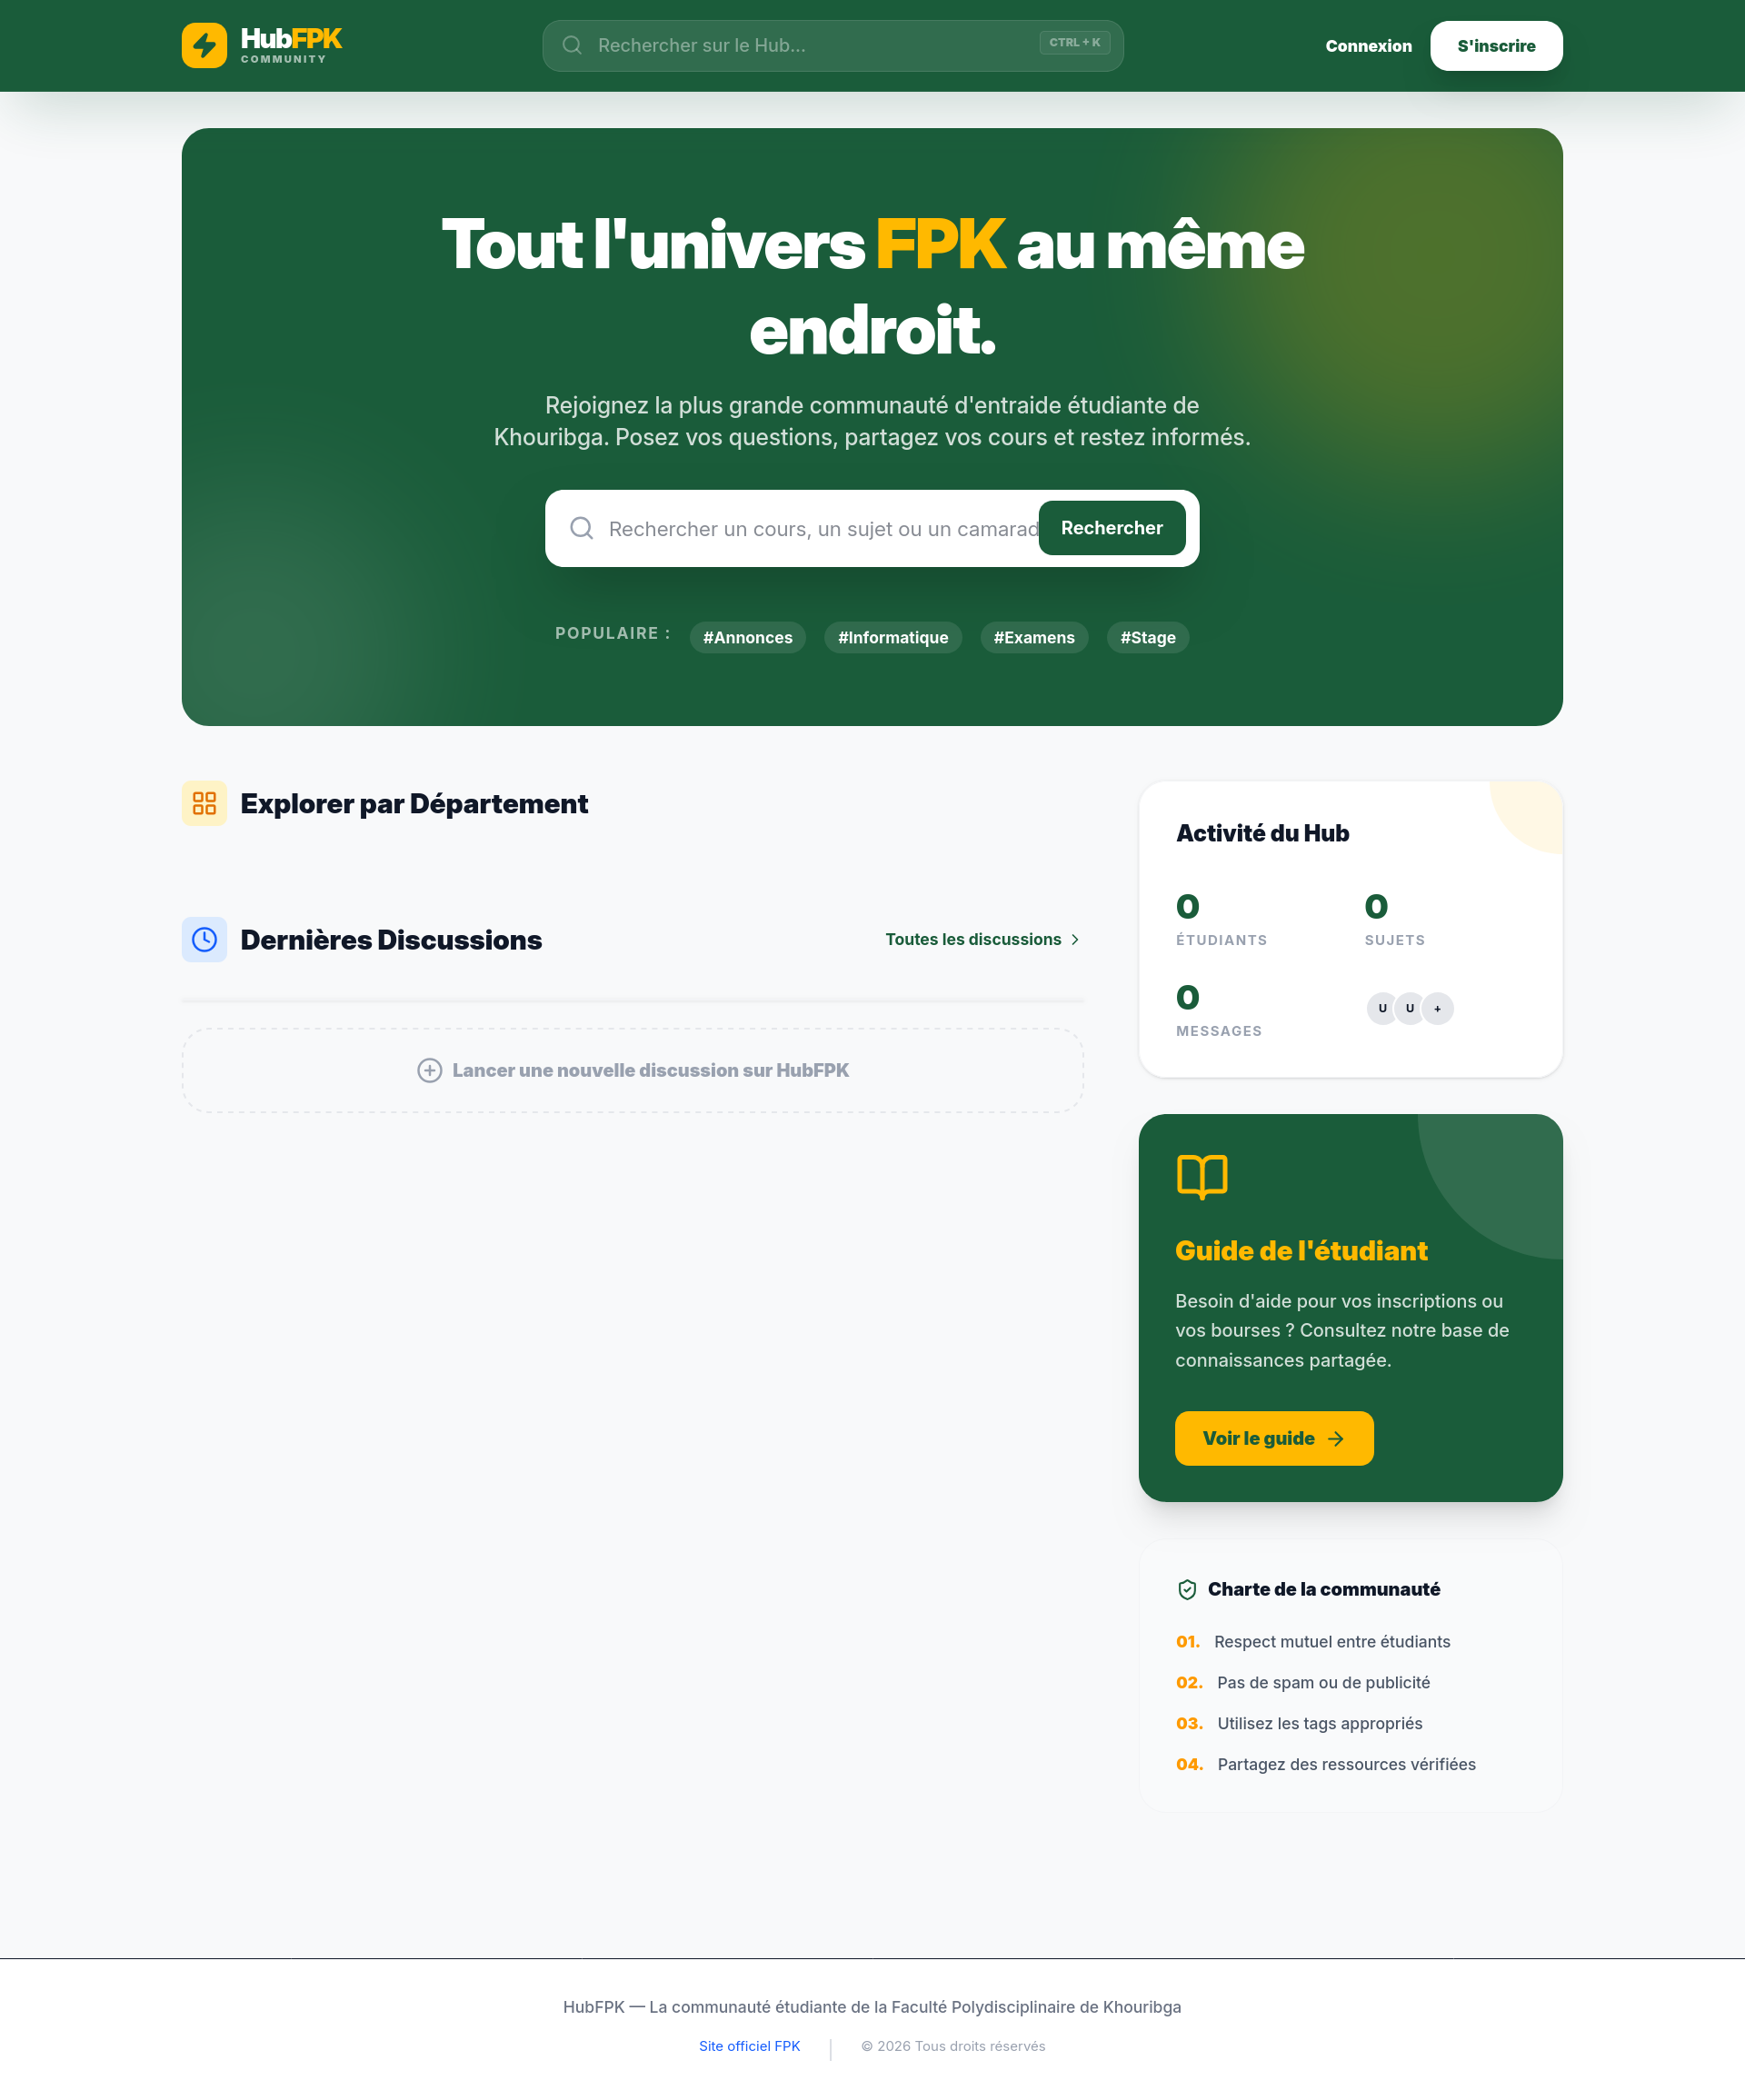
\includegraphics[width=\textwidth]{screens/homePage.png}
    \caption{Page d'accueil de HubFPK. On distingue le hero section avec la barre de recherche, la grille des départements, la liste des discussions récentes et la sidebar avec les statistiques.}
\end{figure}


\subsection{Inscription et Connexion (\texttt{Login.jsx})}

Le composant \texttt{Login.jsx} gère à la fois l'inscription et la connexion selon l'URL (\texttt{/login} ou \texttt{/register}). L'authentification est entièrement déléguée à \textbf{Supabase Auth} :

\begin{itemize}
    \item \textbf{Inscription} : Appel à \texttt{supabase.auth.signUp()} avec email, mot de passe et nom d'utilisateur. Le trigger SQL \texttt{handle\_new\_user()} crée automatiquement le profil.
    \item \textbf{Confirmation par email} : Après inscription, un message invite l'utilisateur à vérifier sa boîte mail pour confirmer son compte.
    \item \textbf{Connexion} : Appel à \texttt{supabase.auth.signInWithPassword()}.
    \item Redirection automatique vers la page d'accueil après succès.
\end{itemize}

\begin{figure}[H]
    \centering
    \begin{subfigure}[b]{0.48\textwidth}
        \centering
        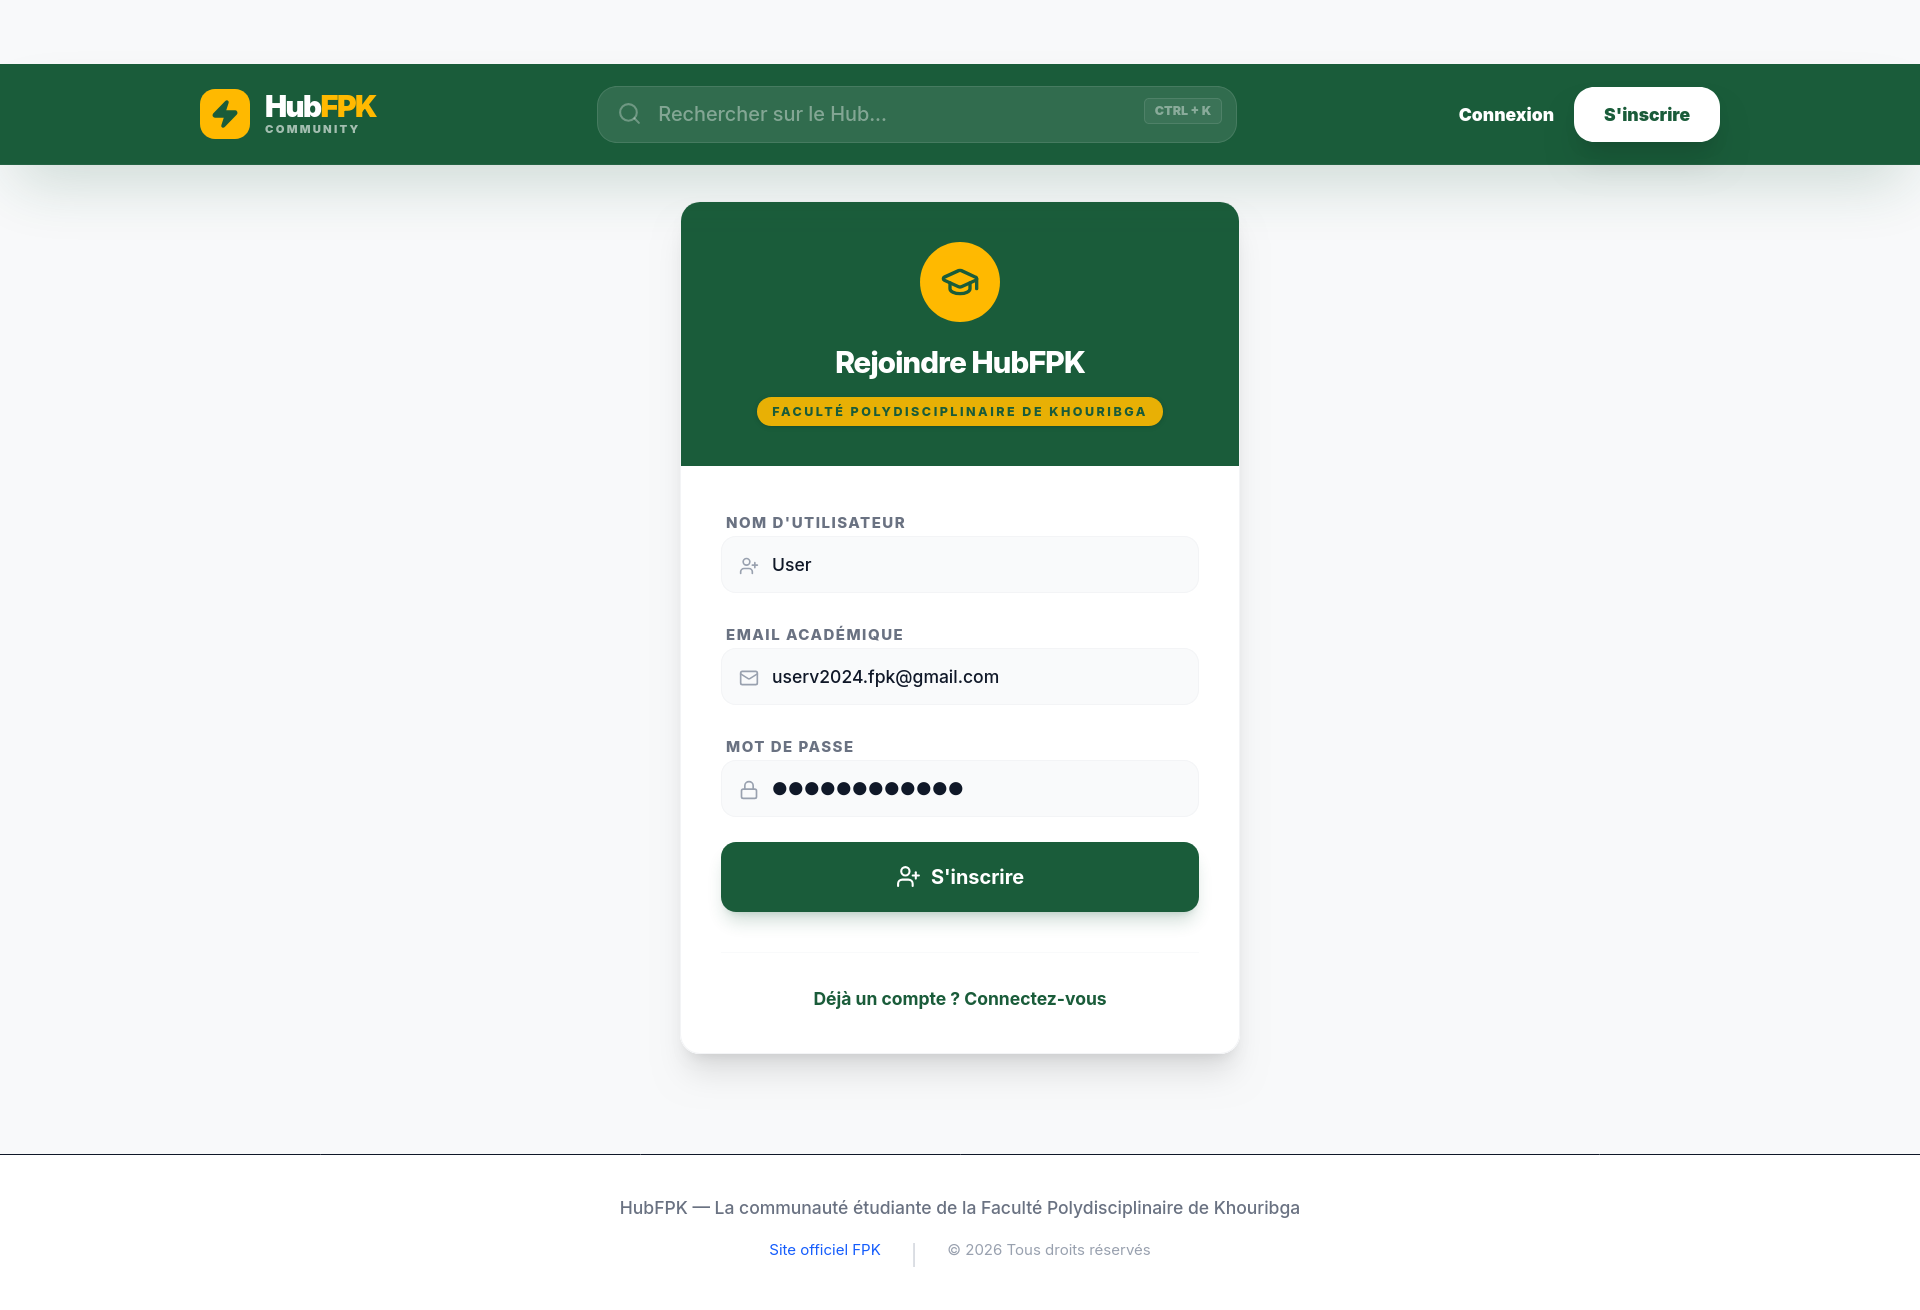
\includegraphics[width=\textwidth]{screens/Account_registration.png}
        \caption{Formulaire d'inscription avec champs email, nom d'utilisateur et mot de passe.}
    \end{subfigure}
    \hfill
    \begin{subfigure}[b]{0.48\textwidth}
        \centering
        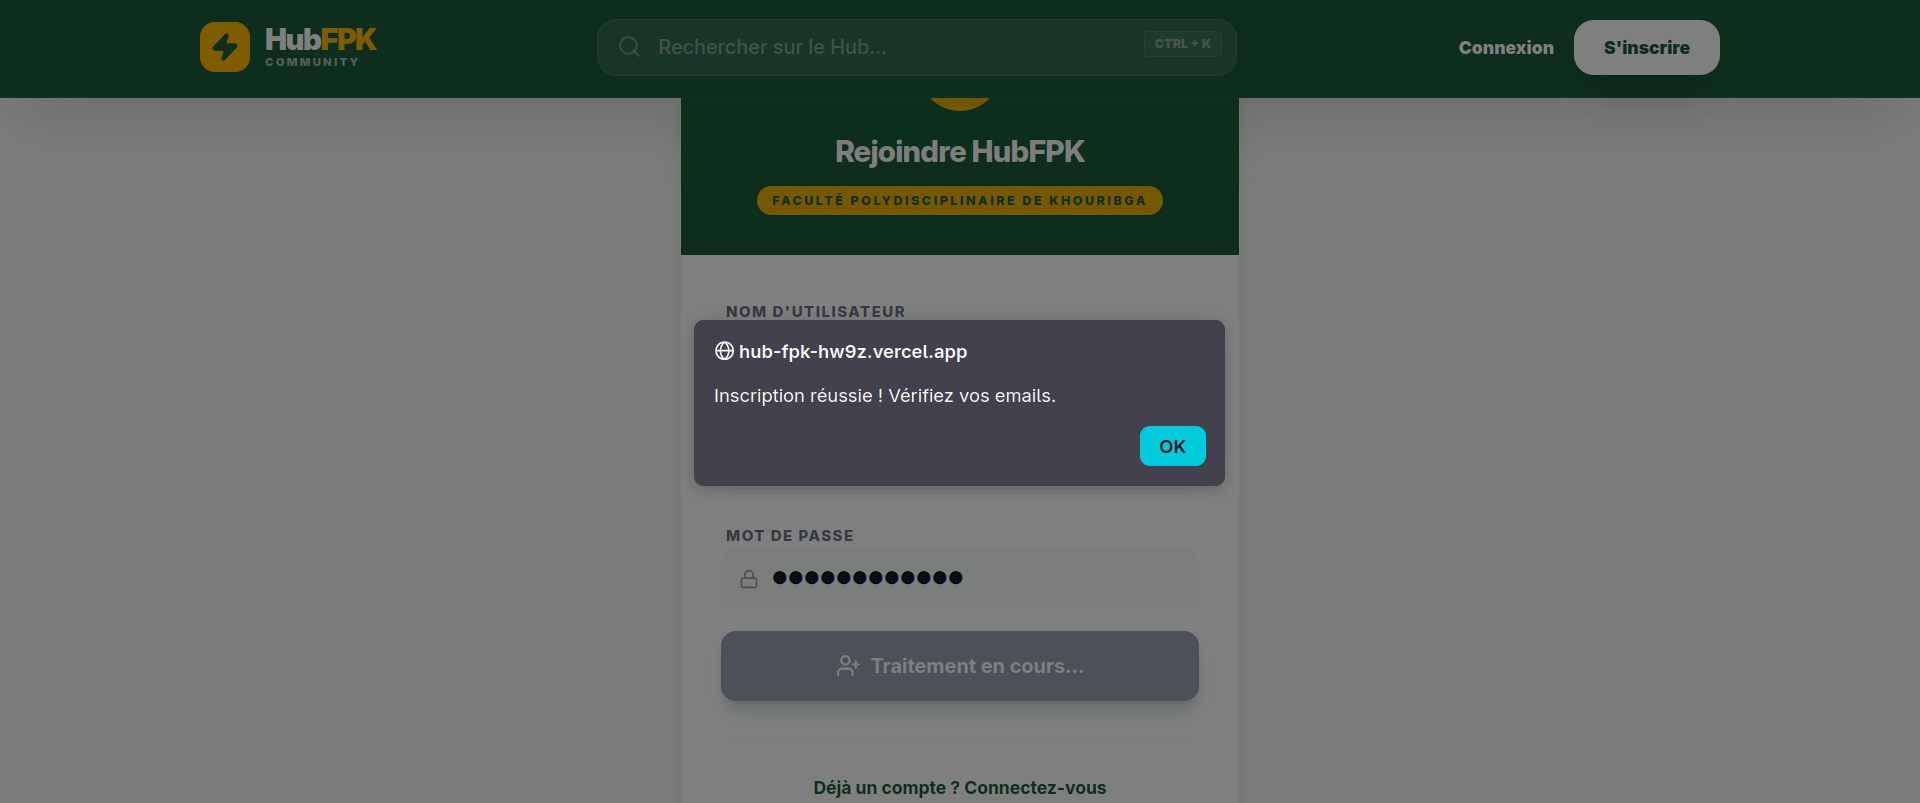
\includegraphics[width=\textwidth]{screens/Account_registration2.png}
        \caption{Message de confirmation invitant l'utilisateur à vérifier son email.}
    \end{subfigure}
    \caption{Processus d'inscription de HubFPK : formulaire et confirmation par email.}
\end{figure}

\begin{figure}[H]
    \centering
    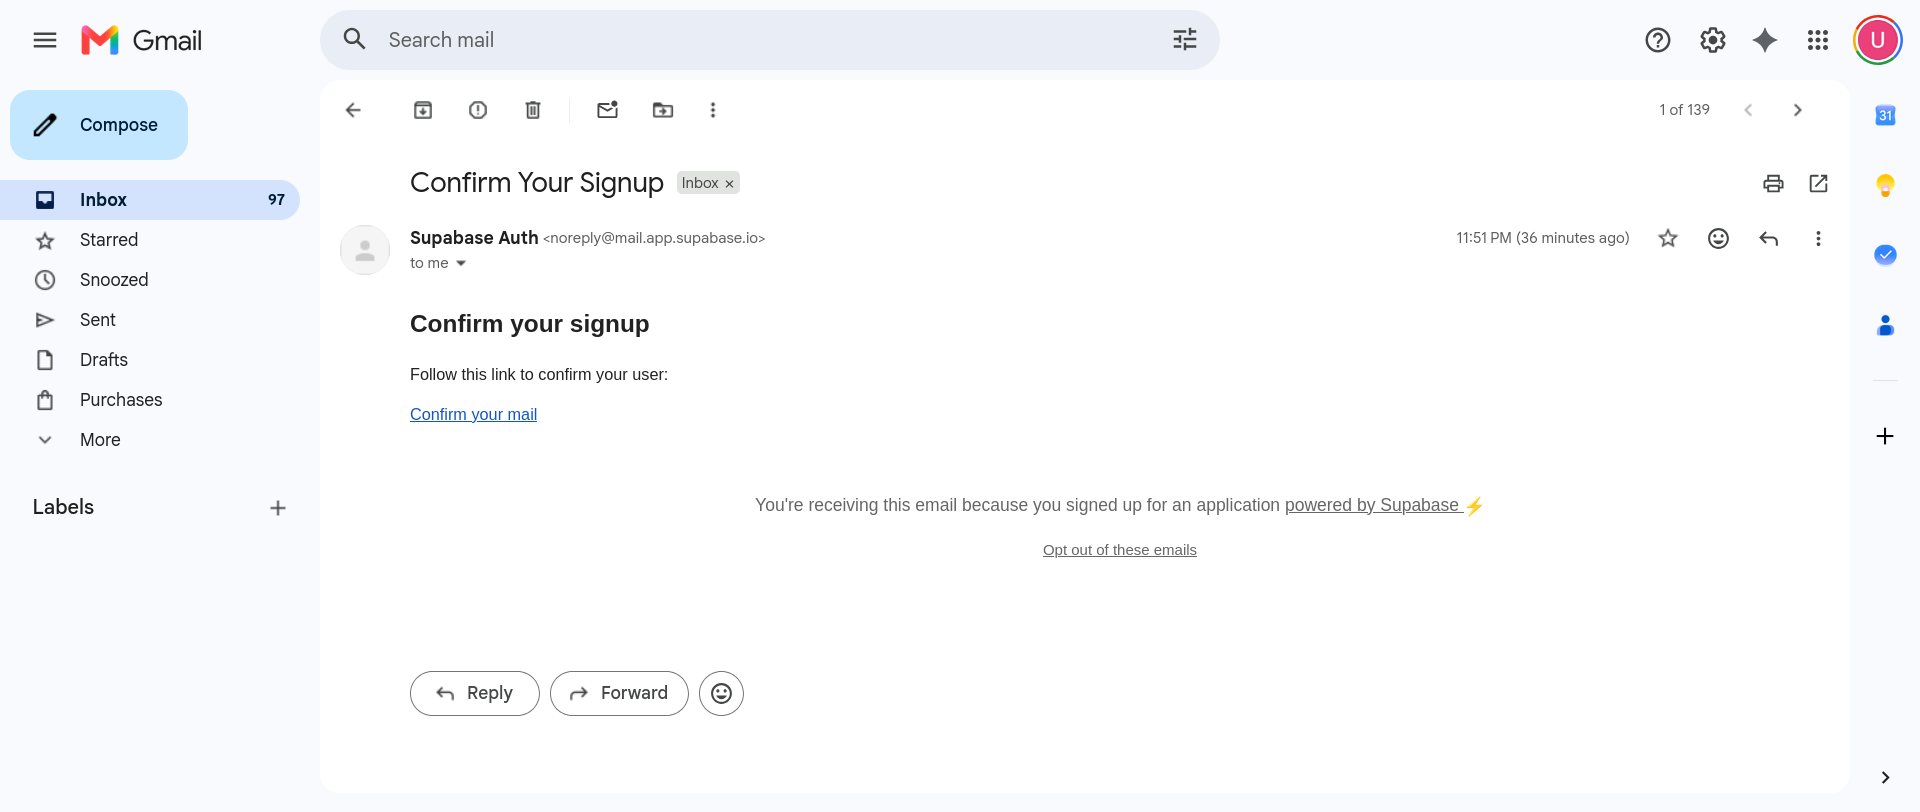
\includegraphics[width=0.7\textwidth]{screens/email_confirmation.png}
    \caption{Email de confirmation reçu dans la boîte de réception de l'utilisateur, permettant de valider son compte HubFPK.}
\end{figure}

\subsection{Création d'une Discussion (\texttt{NewThread.jsx})}

La page de création offre un éditeur complet avec :

\begin{itemize}
    \item \textbf{Titre} : Champ texte pleine largeur.
    \item \textbf{Éditeur / Aperçu Markdown} : Basculement entre le mode éditeur (textarea avec police monospace) et le mode aperçu (rendu via \texttt{react-markdown}).
    \item \textbf{Sélecteur de département} : Dropdown alimenté par l'API \texttt{/api/categories}.
    \item \textbf{Tags} : Sélection visuelle parmi 4 options (Question, Discussion, Ressource, Annonce).
    \item \textbf{Conseils d'écriture} : Encadré jaune avec des bonnes pratiques de rédaction.
\end{itemize}

\begin{figure}[H]
    \centering
    \begin{subfigure}[b]{0.48\textwidth}
        \centering
        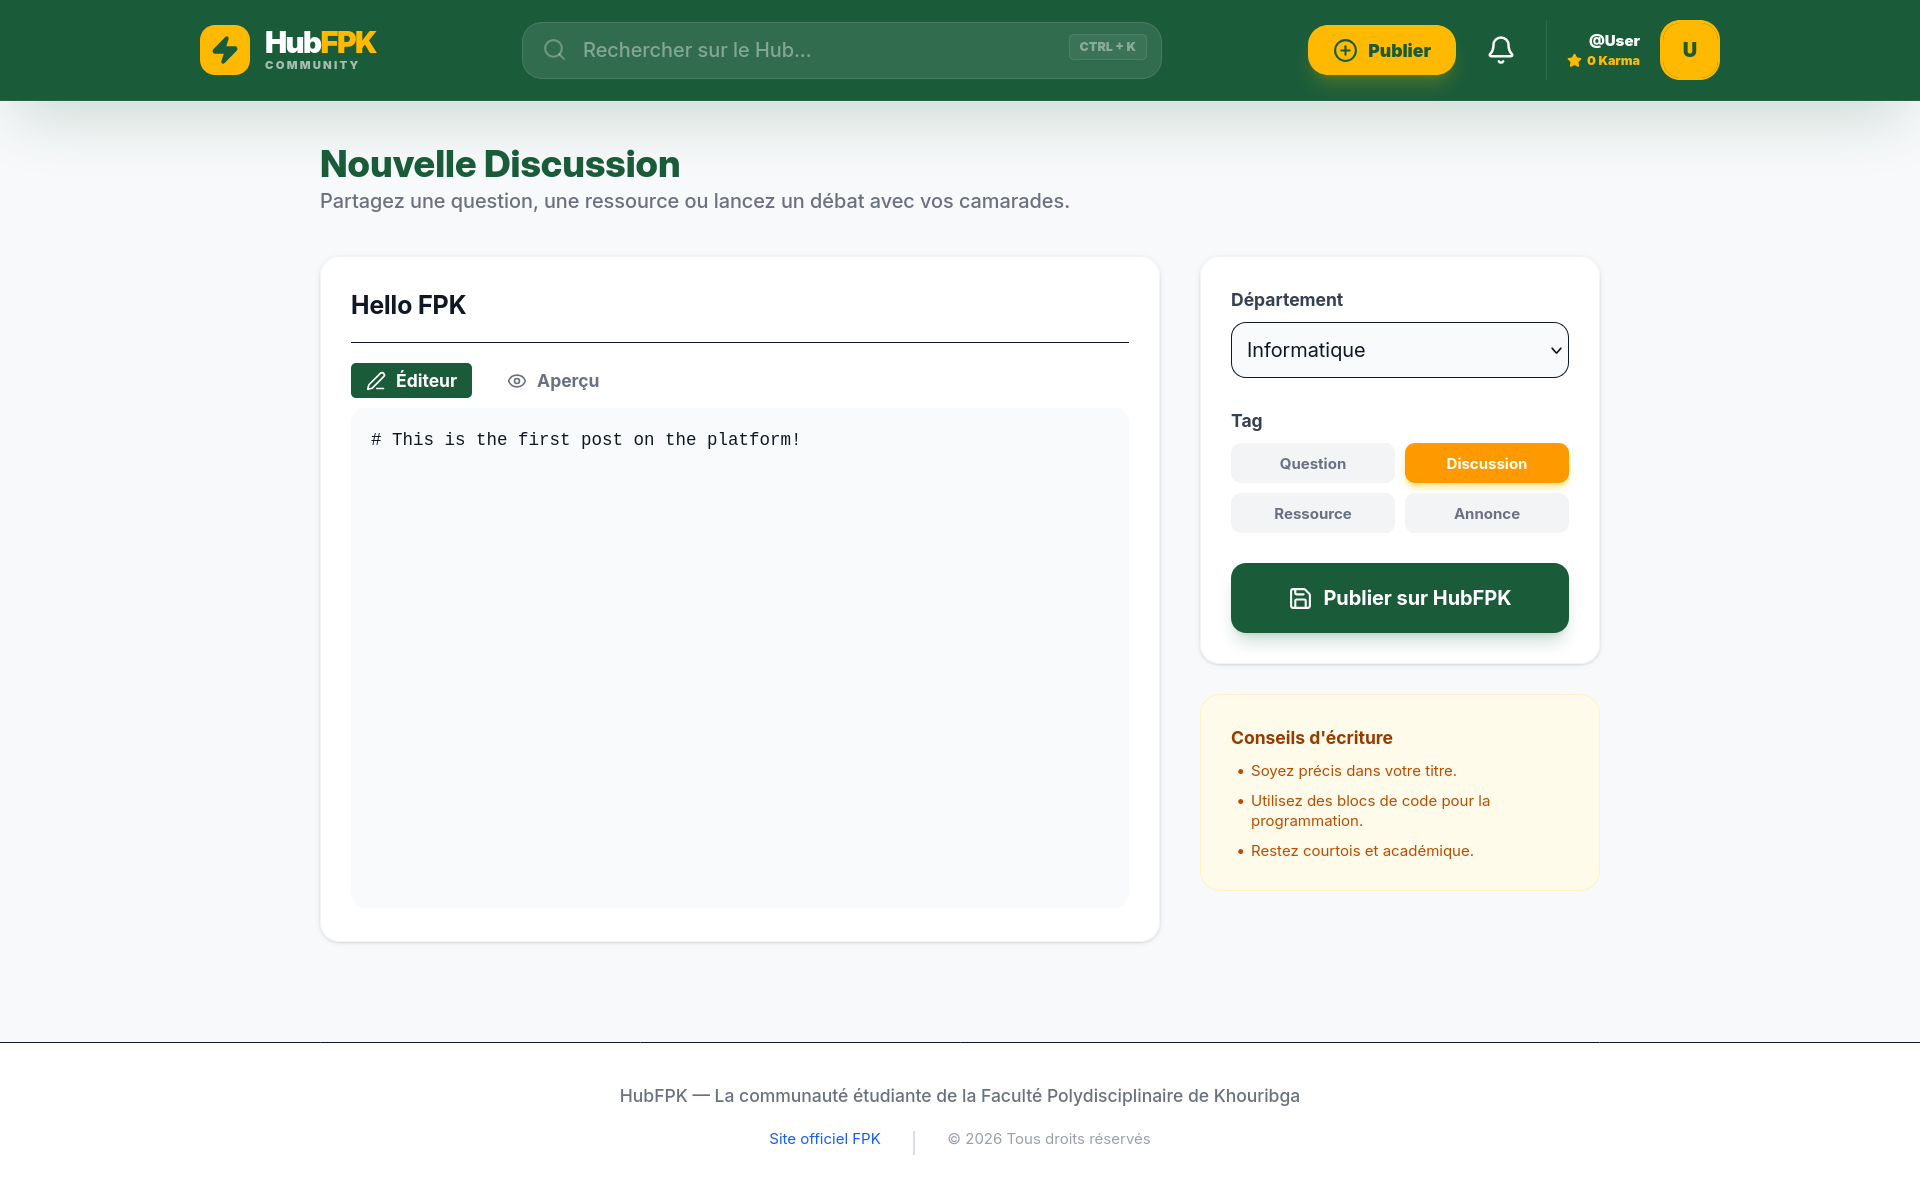
\includegraphics[width=\textwidth]{screens/postCreation1.png}
        \caption{Mode éditeur : rédaction en Markdown avec sélection du département et du tag.}
    \end{subfigure}
    \hfill
    \begin{subfigure}[b]{0.48\textwidth}
        \centering
        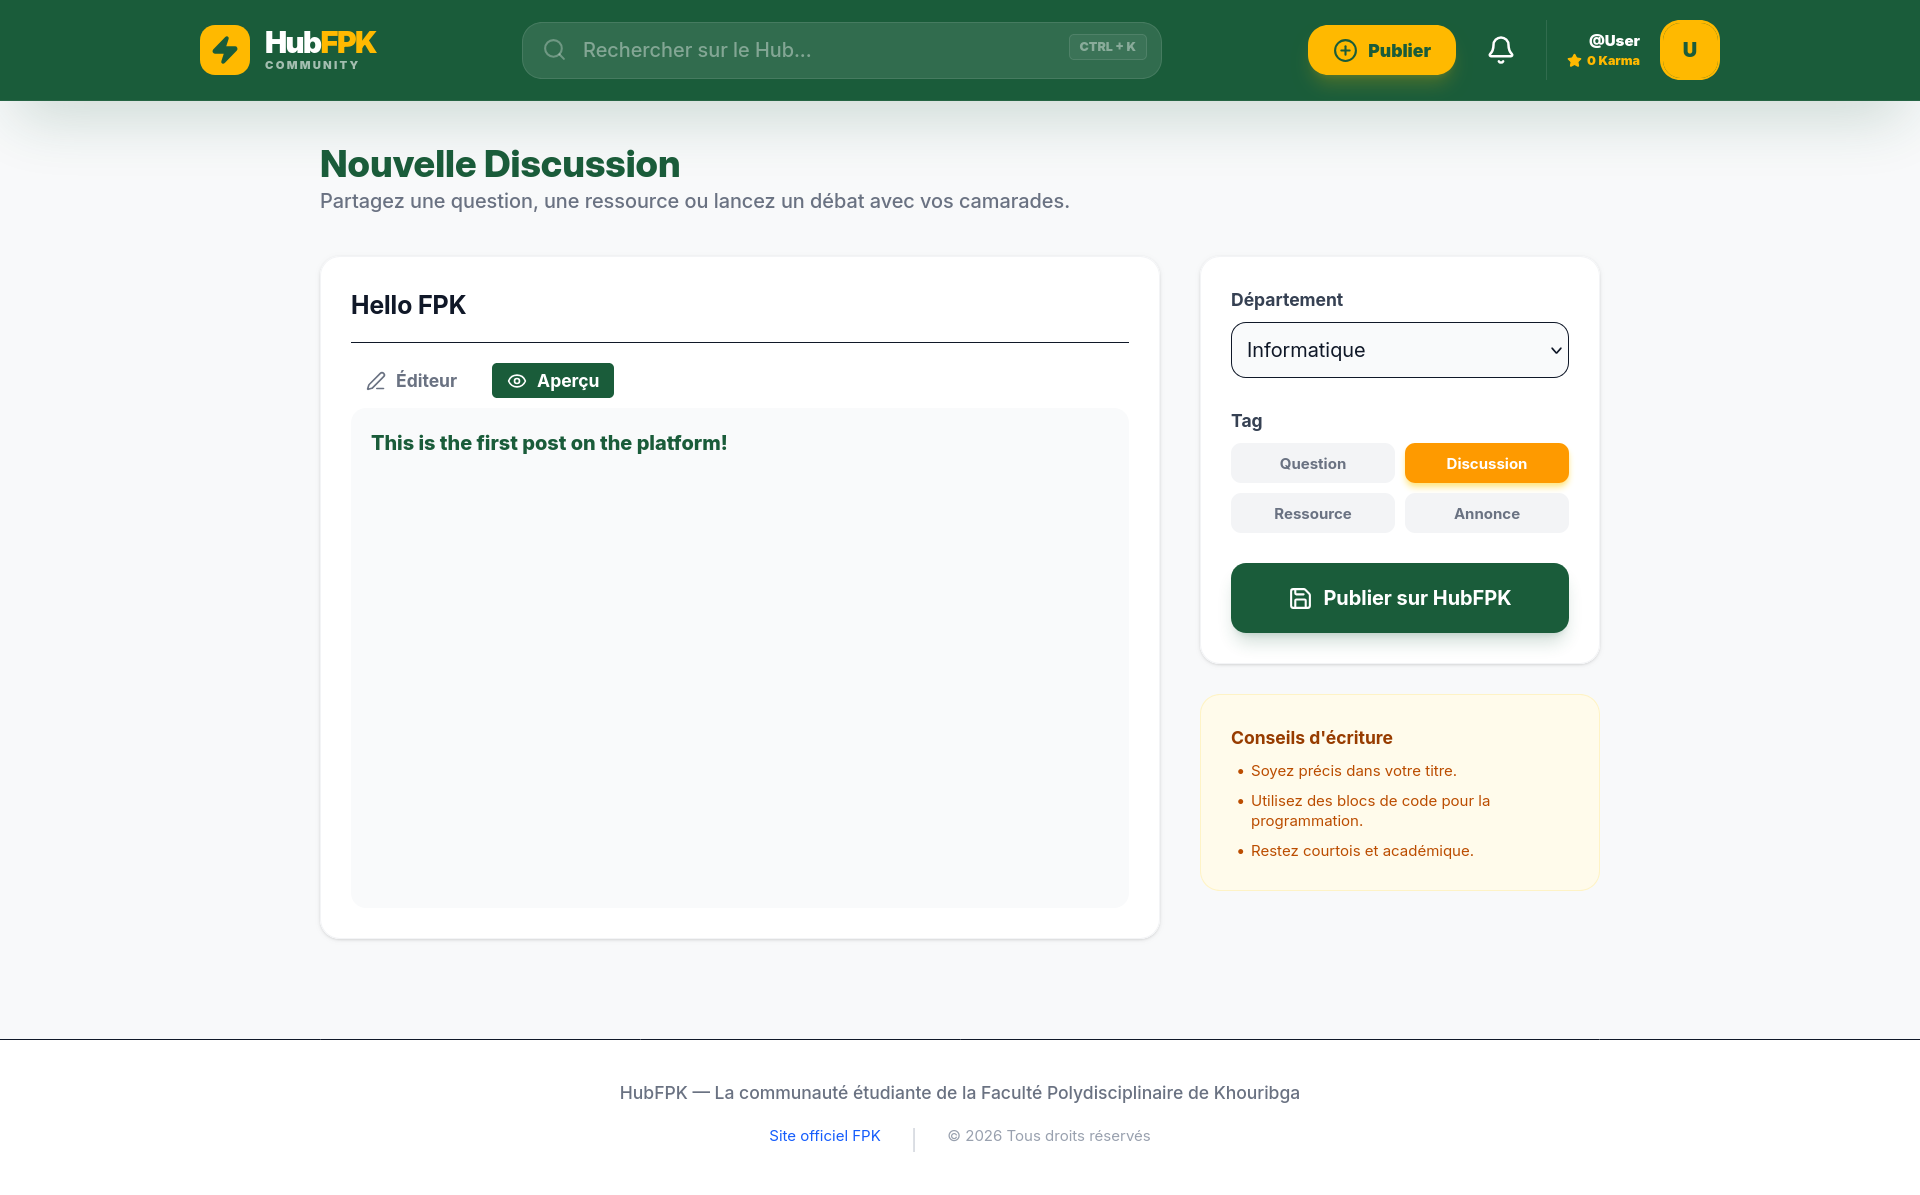
\includegraphics[width=\textwidth]{screens/postCreation2_markdown.png}
        \caption{Mode aperçu : le Markdown est rendu visuellement avant publication.}
    \end{subfigure}
    \caption{Formulaire de création de discussion avec éditeur et aperçu Markdown.}
\end{figure}

\begin{figure}[H]
    \centering
    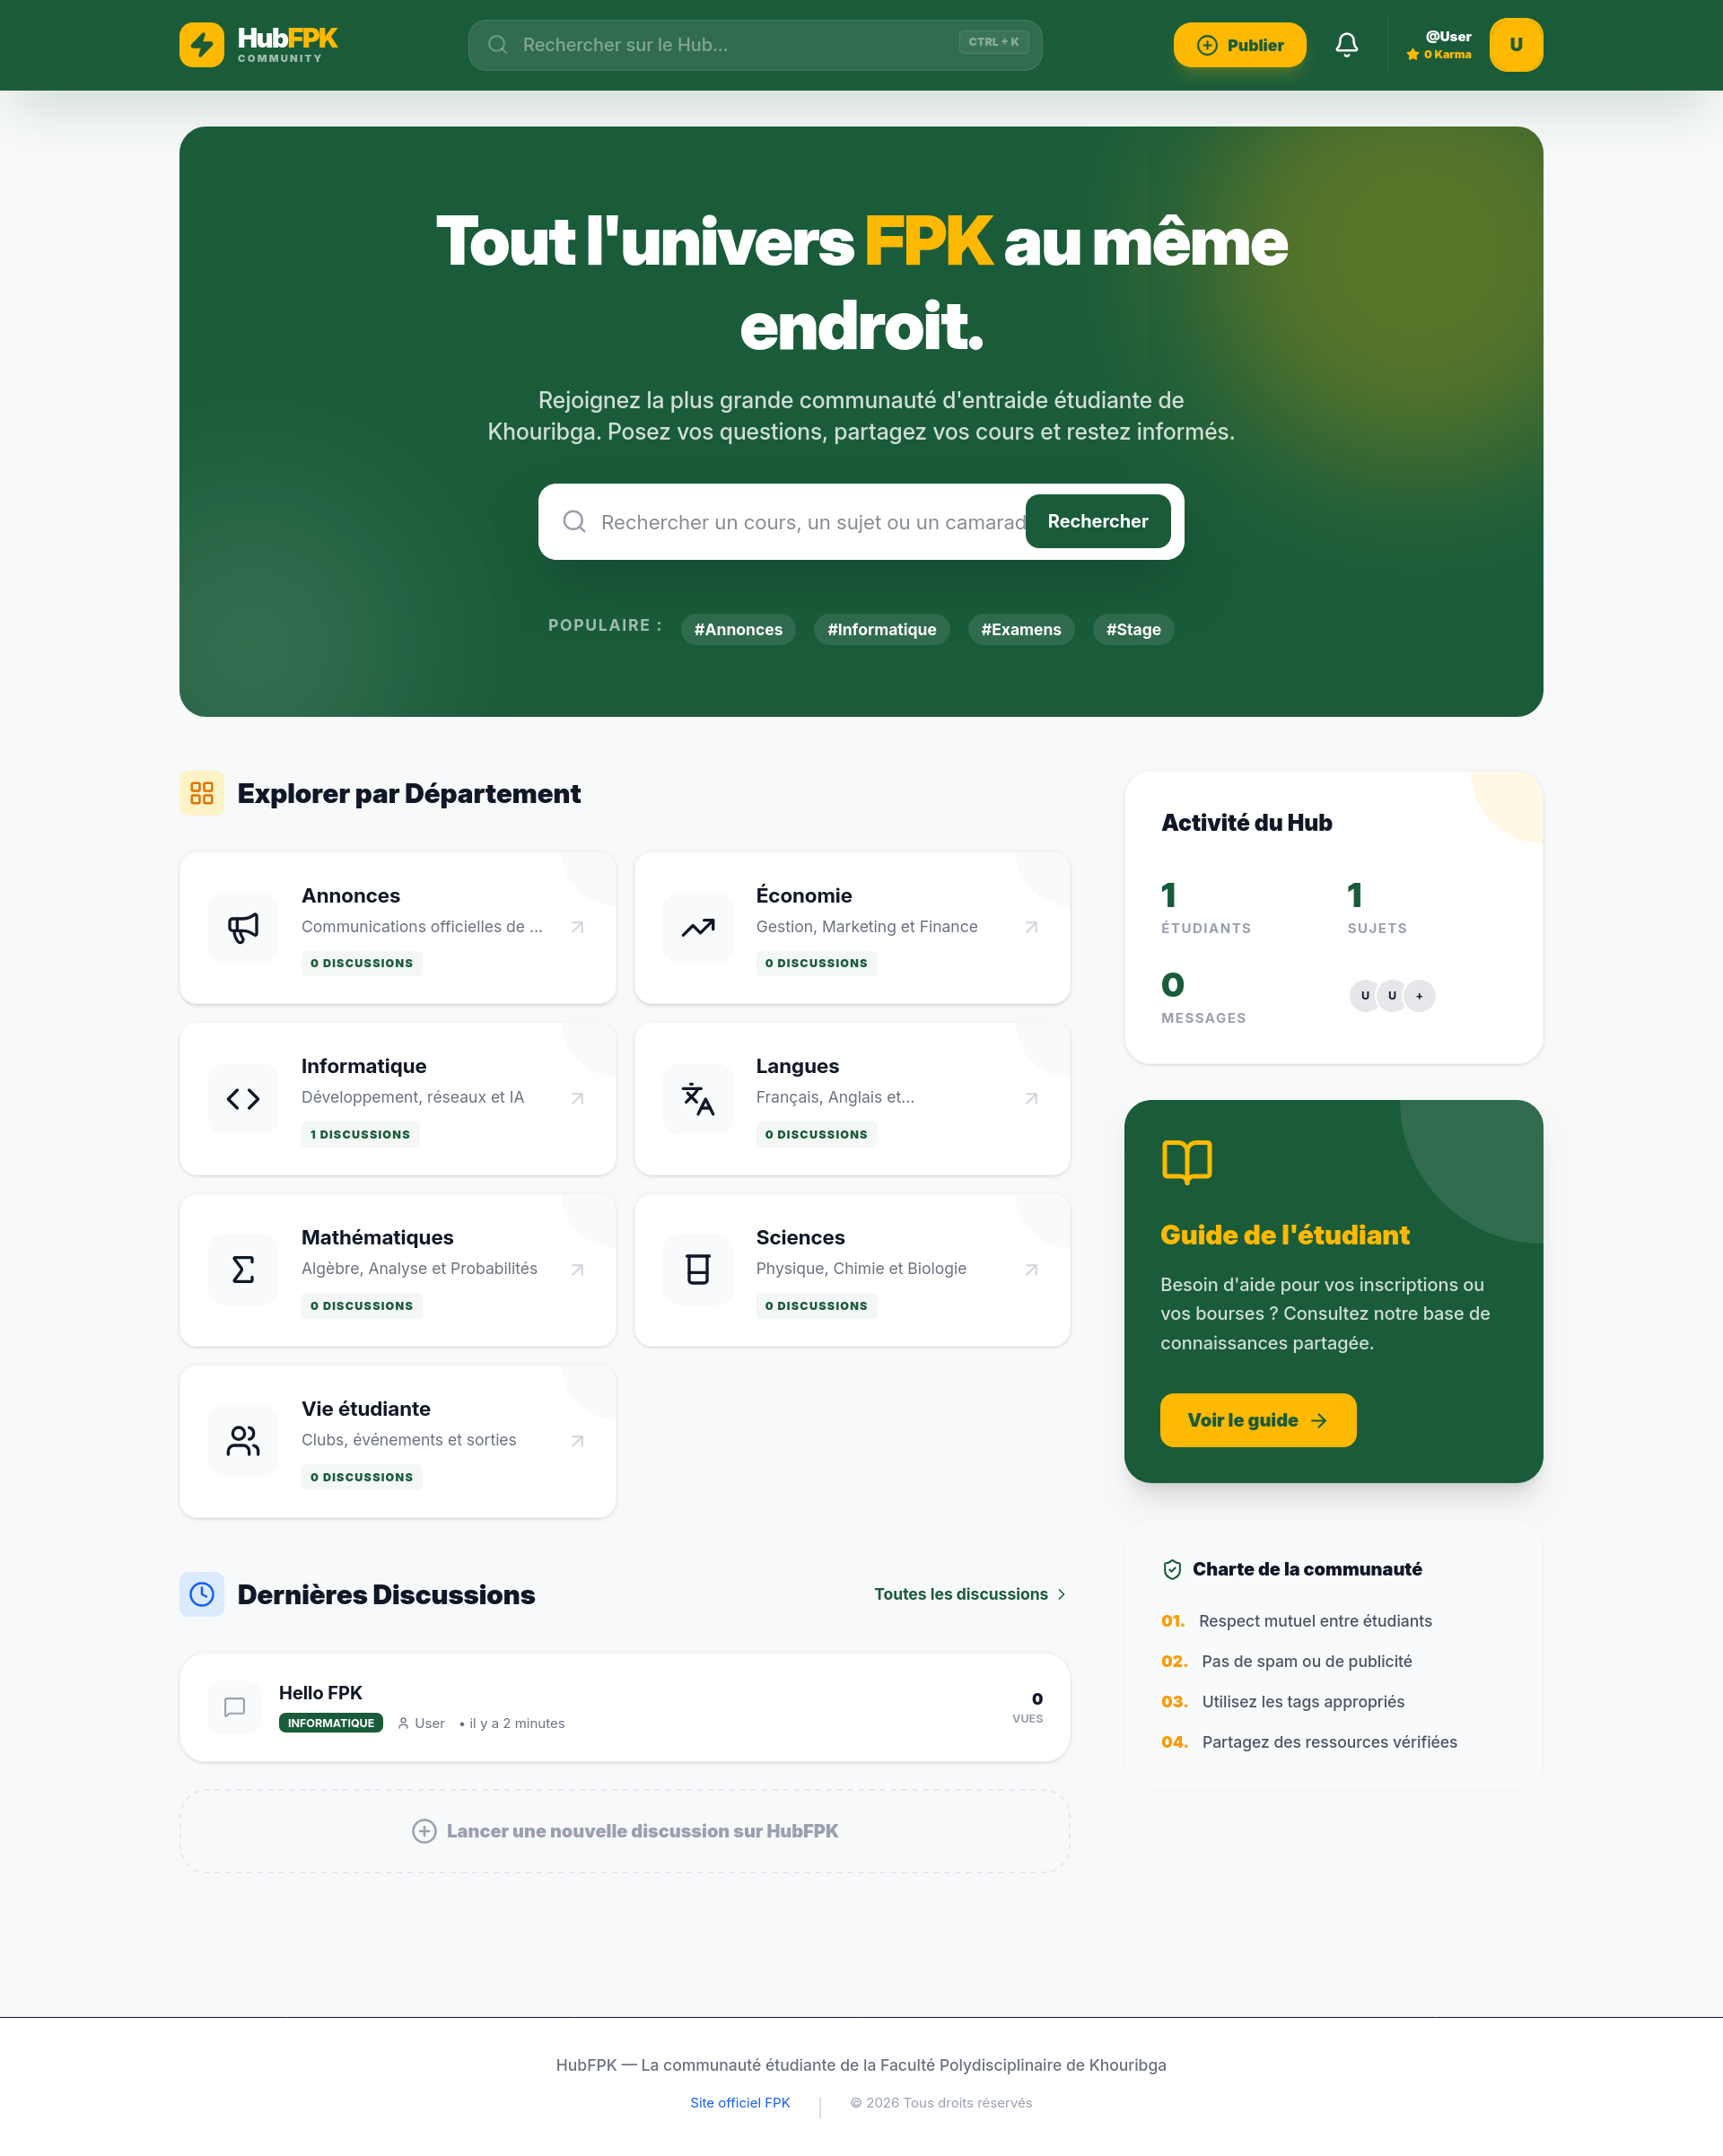
\includegraphics[width=\textwidth]{screens/homepage_after_post.png}
    \caption{Page d'accueil après la publication d'une discussion. Les compteurs de statistiques et la liste des discussions récentes sont mis à jour dynamiquement.}
\end{figure}

\subsection{Vue d'une Discussion (\texttt{ThreadView.jsx})}

La page de visualisation d'un thread est le cœur de l'expérience HubFPK. Elle comprend :

\begin{itemize}
    \item \textbf{En-tête du thread} : Titre, auteur (avec lien vers le profil), catégorie, tag, date relative et compteur de vues.
    \item \textbf{Corps du thread} : Rendu Markdown complet via \texttt{react-markdown}.
    \item \textbf{Système de vote} : Boutons upvote/downvote avec score total calculé dynamiquement. Le vote se fait via le client Supabase JS et met à jour le karma de l'auteur via la procédure stockée \texttt{increment\_karma()}.
    \item \textbf{Réponses imbriquées} : Les réponses sont organisées sur 1 niveau (parent/enfant) avec les profils des répondeurs.
    \item \textbf{Temps réel} : Un canal Supabase Realtime écoute les événements \texttt{INSERT} sur la table \texttt{posts}, permettant de voir les nouvelles réponses apparaître en direct.
    \item \textbf{Bouton de partage} : Copie le lien du thread dans le presse-papier.
\end{itemize}

\begin{figure}[H]
    \centering
    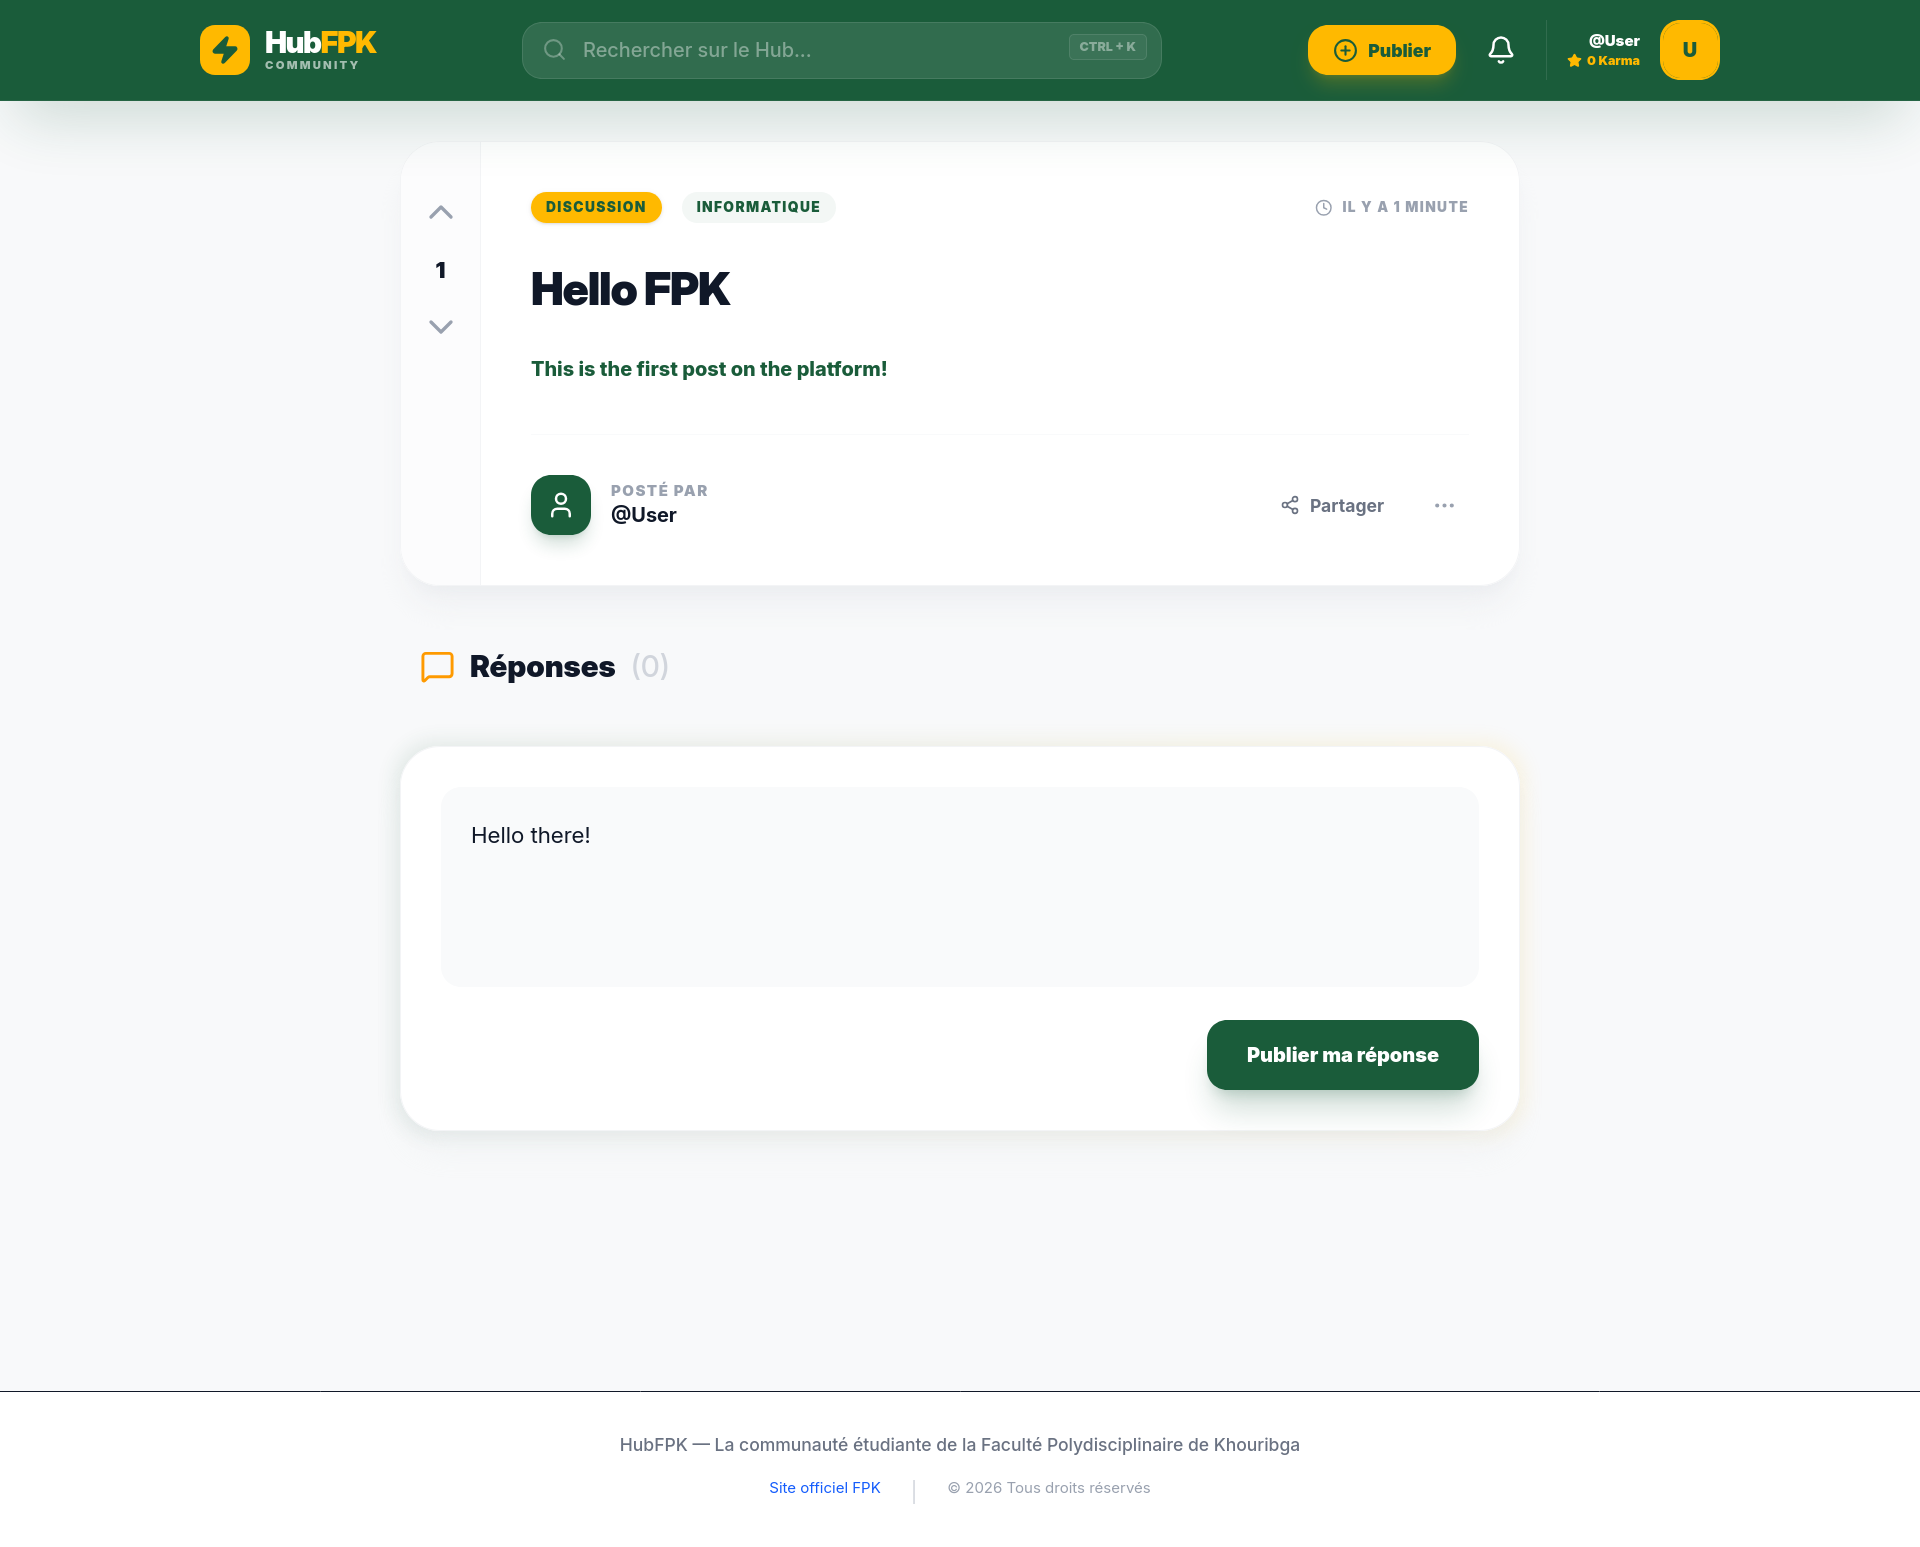
\includegraphics[width=\textwidth]{screens/posted_vote_comment.png}
    \caption{Vue d'un fil de discussion montrant le système de vote (upvote/downvote), le contenu en Markdown et la section de commentaires.}
\end{figure}

\subsection{Barre de Navigation (\texttt{Navbar.jsx})}

La barre de navigation est un composant sticky omniprésent offrant :

\begin{itemize}
    \item \textbf{Logo animé} : ``HubFPK'' avec icône Zap dorée et effet de rotation au survol.
    \item \textbf{Barre de recherche} : Visible sur desktop avec indication du raccourci \texttt{CTRL+K}.
    \item \textbf{Bouton ``Publier''} : Accès rapide à la création de thread (utilisateurs connectés).
    \item \textbf{Dropdown de notifications} : Badge rouge animé (\texttt{animate-bounce}) indiquant les notifications non lues, avec messages contextuels (``Nouvelle réponse'' ou ``Quelqu'un a voté'') et timestamps dynamiques en français.
    \item \textbf{Dropdown de profil} : Affichage du nom d'utilisateur, du karma avec étoile dorée, lien vers le profil et bouton de déconnexion.
\end{itemize}


% ============================================================
% CHAPITRE 6 : DÉPLOIEMENT
% ============================================================
\chapter{Déploiement en Production}

\section{Application en Ligne}

L'application HubFPK est accessible en production à l'adresse suivante :

\begin{center}
\Large\sffamily\bfseries
\url{https://hub-fpk-hw9z.vercel.app/}
\end{center}

L'API backend est quant à elle accessible à l'adresse : \url{https://hub-fpk.vercel.app/}.

\section{Choix de Vercel}

Le déploiement de HubFPK a été réalisé sur \textbf{Vercel}, une plateforme cloud spécialisée dans l'hébergement d'applications web modernes. Ce choix offre plusieurs avantages :

\begin{itemize}
    \item \textbf{Déploiement automatique} : Chaque push sur le dépôt GitHub déclenche un redéploiement automatique (\textit{Continuous Deployment}).
    \item \textbf{Serverless Functions} : Le backend Express est automatiquement transformé en fonctions serverless, éliminant le besoin de gérer un serveur dédié.
    \item \textbf{CDN mondial} : Les fichiers statiques du frontend sont distribués via un réseau de diffusion de contenu (CDN) pour des temps de chargement minimaux.
    \item \textbf{HTTPS automatique} : Tous les domaines Vercel bénéficient d'un certificat SSL gratuit.
    \item \textbf{Gratuité} : Le plan gratuit de Vercel est suffisant pour un projet académique.
\end{itemize}

\section{Architecture de Déploiement}

Le projet est déployé en \textbf{deux projets Vercel distincts} :

\begin{table}[H]
\centering
\renewcommand{\arraystretch}{1.3}
\begin{tabularx}{\textwidth}{l l l X}
\toprule
\textbf{Composant} & \textbf{URL} & \textbf{Preset} & \textbf{Variables clés} \\
\midrule
Backend & \texttt{hub-fpk.vercel.app} & Express & \texttt{SUPABASE\_URL}, \texttt{SUPABASE\_KEY}, \texttt{FRONTEND\_URL} \\
Frontend & \texttt{hub-fpk-hw9z.vercel.app} & Vite & \texttt{VITE\_API\_URL}, \texttt{VITE\_SUPABASE\_URL}, \texttt{VITE\_SUPABASE\_ANON\_KEY} \\
\bottomrule
\end{tabularx}
\caption{Configuration de déploiement des deux projets Vercel.}
\end{table}

\section{Configuration CORS}

Un point crucial du déploiement est la configuration correcte du \textbf{CORS} (Cross-Origin Resource Sharing). Le backend doit explicitement autoriser les requêtes provenant du domaine du frontend :

\begin{lstlisting}[language=JavaScript, caption={Configuration CORS dans le backend.}]
app.use(cors({
  origin: process.env.FRONTEND_URL,
  credentials: true
}));
\end{lstlisting}

La variable d'environnement \texttt{FRONTEND\_URL} doit correspondre exactement à l'URL du frontend déployé (\textbf{sans slash final}), faute de quoi les requêtes seront bloquées par le navigateur.

\section{Procédure de Déploiement}

\begin{enumerate}
    \item \textbf{Préparer le code source} : S'assurer que le code est poussé sur le dépôt GitHub.
    \item \textbf{Créer le projet backend sur Vercel} : Importer le dépôt GitHub, sélectionner le framework preset ``Express'', définir le \textit{Root Directory} sur \texttt{forum-backend}, et configurer les variables d'environnement Supabase.
    \item \textbf{Créer le projet frontend sur Vercel} : Même processus avec le preset ``Vite'', \textit{Root Directory} sur \texttt{forum-frontend}, et les variables d'environnement frontend.
    \item \textbf{Configurer le CORS} : Ajouter la variable \texttt{FRONTEND\_URL} dans le projet backend pointant vers l'URL du frontend, puis redéployer le backend.
    \item \textbf{Vérifier} : Tester l'application en production pour s'assurer que toutes les fonctionnalités (auth, CRUD, notifications) fonctionnent correctement.
\end{enumerate}


% ============================================================
% CHAPITRE 7 : ANALYSE CRITIQUE
% ============================================================
\chapter{Analyse Critique du Projet}

Une analyse approfondie du projet a été réalisée afin d'évaluer sa maturité technique et d'identifier les axes d'amélioration prioritaires.

\section{Sécurité}

\subsection{Points Positifs}

\begin{itemize}
    \item Supabase RLS activé sur \textbf{toutes les tables} sans exception.
    \item Authentification déléguée à \textbf{Supabase Auth}, un standard de sécurité élevé (bcrypt, tokens JWT).
    \item Variables d'environnement utilisées pour tous les secrets (clés API, URL de la base).
    \item Fichiers \texttt{.env.example} fournis pour faciliter la configuration.
\end{itemize}

\subsection{Vulnérabilités Identifiées}

\begin{table}[H]
\centering
\renewcommand{\arraystretch}{1.3}
\begin{tabularx}{\textwidth}{l l X}
\toprule
\textbf{Vulnérabilité} & \textbf{Impact} & \textbf{Recommandation} \\
\midrule
CORS ouvert & N'importe quel domaine peut appeler l'API & Restreindre à l'URL du frontend \\
\texttt{user\_id} dans le body POST & Usurpation d'identité & Extraire \texttt{user\_id} depuis le JWT côté serveur \\
Aucune validation des entrées & XSS, données corrompues & Utiliser Zod ou Joi \\
Pas de rate limiting & Brute-force, spam & Ajouter \texttt{express-rate-limit} \\
Email non validé & Comptes non-étudiants & Valider le domaine \texttt{@fpk.ac.ma} \\
\bottomrule
\end{tabularx}
\caption{Vulnérabilités de sécurité identifiées et recommandations associées.}
\end{table}

\textbf{Note :} Lors du développement, la vulnérabilité CORS a été corrigée en restreignant l'origine aux seules requêtes provenant du frontend via la variable \texttt{FRONTEND\_URL}.

\section{Performance}

\subsection{Forces}

\begin{itemize}
    \item \textbf{Chargements parallèles} avec \texttt{Promise.all()} dans la page d'accueil et les routes backend.
    \item \textbf{Skeleton loading} pour améliorer l'UX perçue pendant le chargement des données.
    \item \textbf{Realtime via WebSocket} Supabase, évitant tout mécanisme de polling coûteux.
    \item \textbf{\texttt{useCallback}} pour stabiliser les fonctions dépendantes et éviter les re-renders inutiles.
\end{itemize}

\subsection{Faiblesses}

\begin{itemize}
    \item \textbf{Problème N+1} dans \texttt{/api/categories} : une requête supplémentaire est effectuée pour chaque catégorie afin de compter ses threads, au lieu d'utiliser un \texttt{GROUP BY} ou une vue SQL.
    \item \textbf{Pas de pagination réelle} : toutes les données sont chargées en une seule fois.
    \item \textbf{Re-fetch complet} du thread à chaque événement Realtime, au lieu de n'ajouter que le nouveau post.
    \item \textbf{Pas de cache client} (React Query ou SWR) pour éviter les requêtes redondantes.
    \item \textbf{Import global} \texttt{* as LucideIcons} dans \texttt{Home.jsx} et \texttt{CategoryView.jsx}, impactant la taille du bundle.
\end{itemize}

\section{Qualité du Code}

\subsection{Points Positifs}

\begin{itemize}
    \item Code bien structuré, lisible et organisé par domaine fonctionnel.
    \item Commentaires pertinents dans les fichiers clés.
    \item Composant \texttt{Skeleton} réutilisable pour les états de chargement.
    \item Gestion des états vides et des erreurs avec des interfaces dédiées.
\end{itemize}

\subsection{Points à Améliorer}

\begin{itemize}
    \item Pas de tests unitaires ni de tests d'intégration.
    \item \texttt{API\_URL} dupliqué dans chaque page (pas de module centralisé \texttt{api.js}).
    \item Logique de notifications dupliquée entre le backend Node.js et les triggers SQL.
    \item Pas de TypeScript pour le typage statique.
    \item Pas de configuration ESLint/Prettier côté backend.
\end{itemize}

\section{Corrections Appliquées}

Au cours du développement, plusieurs bugs et problèmes ont été identifiés et corrigés :

\begin{itemize}
    \item \checkmark\ CORS restreint à l'URL du frontend via \texttt{FRONTEND\_URL}.
    \item \checkmark\ Route \texttt{/leaderboard/top} réparée (conflit de routage avec \texttt{/:username} dans Express).
    \item \checkmark\ Timestamps de notifications rendus dynamiques via \texttt{date-fns} avec locale française.
    \item \checkmark\ Bouton ``Tout marquer lu'' rendu fonctionnel.
    \item \checkmark\ Messages de notification contextuels (``Nouvelle réponse'' vs. ``Quelqu'un a voté'').
    \item \checkmark\ Fichier \texttt{App.css} nettoyé du boilerplate Vite inutilisé.
    \item \checkmark\ Variable \texttt{FRONTEND\_URL} ajoutée aux fichiers \texttt{.env} et \texttt{.env.example}.
\end{itemize}

\section{Synthèse d'Évaluation}

\begin{table}[H]
\centering
\renewcommand{\arraystretch}{1.4}
\begin{tabularx}{\textwidth}{l c X}
\toprule
\textbf{Aspect} & \textbf{Score} & \textbf{Commentaire} \\
\midrule
Architecture & 7/10 & Découplée et claire, double voie d'accès BDD à harmoniser \\
Fonctionnalités & 7/10 & Bon c\oe{}ur fonctionnel, bugs critiques corrigés \\
Sécurité & 5/10 & CORS corrigé, authentification backend reste à implémenter \\
Performance & 6/10 & Bonnes pratiques de base, problème N+1 à corriger \\
UI/UX & 8/10 & Design moderne, cohérent, animations et skeleton loading \\
Qualité de code & 7/10 & Lisible, boilerplate nettoyé, bugs fixés \\
Base de données & 7/10 & Schéma bien pensé, RLS activé, quelques FK manquantes \\
\bottomrule
\end{tabularx}
\caption{Synthèse d'évaluation globale du projet HubFPK (sur 10).}
\end{table}


% ============================================================
% CHAPITRE 8 : CONCLUSION ET PERSPECTIVES
% ============================================================
\chapter{Conclusion et Perspectives}

\section{Bilan du Projet}

Le projet \textbf{HubFPK} représente une solution complète et fonctionnelle de forum communautaire académique. En couvrant l'intégralité de la chaîne -- de la conception du schéma relationnel PostgreSQL à la création d'une API RESTful, en passant par le développement d'une interface React moderne et le déploiement en production sur Vercel -- ce projet démontre une maîtrise des compétences \textit{Full-Stack} modernes.

Les points forts majeurs du projet sont :

\begin{itemize}
    \item \textbf{L'architecture découplée} entre frontend et backend via l'API REST, permettant une évolution indépendante de chaque couche.
    \item \textbf{Le système de votes et de karma}, directement inspiré de Reddit, qui encourage la qualité des contributions.
    \item \textbf{Les notifications en temps réel} via Supabase Realtime (WebSocket), offrant une expérience utilisateur dynamique sans polling.
    \item \textbf{L'éditeur Markdown} avec aperçu en direct, permettant des publications riches et bien formatées.
    \item \textbf{La sécurité} via Row Level Security (RLS) au niveau PostgreSQL, le CORS restreint et l'authentification Supabase Auth.
    \item \textbf{Le déploiement cloud} sur Vercel, rendant la plateforme accessible en ligne à tous les étudiants de la FPK.
\end{itemize}

\section{Fonctionnalités Implémentées}

\begin{itemize}
    \item Inscription et connexion sécurisées (email/mot de passe)
    \item Profil utilisateur avec karma, threads et posts
    \item 7 catégories (départements) avec icônes dynamiques
    \item Création de threads avec tags et support Markdown
    \item Réponses imbriquées sur 1 niveau
    \item Système de vote ±1 (toggle) avec calcul de karma
    \item Notifications en temps réel (réponses + votes)
    \item Recherche par titre de discussion
    \item Compteur de vues par thread
    \item Threads épinglés (pinned)
    \item Skeleton loading pour une meilleure UX
    \item Partage de lien (copie dans le presse-papier)
    \item Leaderboard des utilisateurs par karma
\end{itemize}

\section{Perspectives d'Amélioration}

Pour faire évoluer HubFPK au-delà du cadre scolaire, plusieurs pistes peuvent être explorées :

\begin{itemize}
    \item \textbf{Sécurisation complète du backend} : Ajouter un middleware d'authentification JWT qui vérifie et extrait le \texttt{user\_id} automatiquement depuis le token, au lieu de le recevoir dans le corps de la requête.
    \item \textbf{Validation des entrées} : Intégrer une bibliothèque comme \texttt{Zod} ou \texttt{Joi} pour valider et sanitiser toutes les données reçues par l'API.
    \item \textbf{Pagination} : Implémenter une pagination côté API et frontend pour gérer un grand nombre de discussions.
    \item \textbf{Validation email académique} : Restreindre l'inscription aux adresses \texttt{@fpk.ac.ma} pour garantir que seuls les étudiants de la FPK accèdent à la plateforme.
    \item \textbf{Dark Mode} : Ajouter un mode sombre pour améliorer le confort de lecture.
    \item \textbf{Notifications Push} : Intégrer des notifications push via les \textit{Service Workers} pour alerter les étudiants même lorsqu'ils ne sont pas sur la plateforme.
    \item \textbf{Upload d'images et d'avatars} : Permettre aux étudiants de personnaliser leur profil et d'illustrer leurs publications.
    \item \textbf{Modération} : Implémenter un système de signalement et de modération par les pairs ou par des administrateurs désignés.
    \item \textbf{Tests automatisés} : Ajouter des tests unitaires (Vitest pour le frontend, Jest/Supertest pour le backend) et des tests d'intégration.
    \item \textbf{Application mobile} : Développer une version mobile avec React Native ou Flutter pour une expérience optimale sur smartphone.
\end{itemize}

\vspace{1cm}
\noindent\rule{\textwidth}{0.5pt}
\begin{center}
    \textit{Ce rapport a été rédigé dans le cadre du module \textbf{Citoyenneté et Initiation}, encadré par \textbf{M. CHAKRAOUI Mohamed}.}
\end{center}

\end{document}
